\emph{{\bfseries Информационно-коммуникационные и химические технологии}}
Стр.

{\bfseries Даркенбаев Д.К., Зиятбекова Г.З. , Алтыбай А., Мекебаев Н.О.,
Жамангарин Д.С.}

\emph{ИССЛЕДОВАНИЕ СИСТЕМ КРЕДИТНОГО СКОРИНГА С ИСПОЛЬЗОВАНИЕМ
АЛГОРИТМОВ МАШИННОГО
ОБУЧЕНИЯ..............................................................................................................................}

{\bfseries Akishev K., Тulegulov А., Zhamangarin D., Nurtai Z., Ospanov E.}

\emph{EVALUATION OF THE EFFECTIVENESS OF USING THE SOFTWARE PRODUCT
"ASSISTANT FOR}

\emph{THE PREPARATION OF TEST TASKS" TO TEST THE KNOWLEDGE OF
STUDENTS\ldots\ldots\ldots\ldots\ldots\ldots\ldots\ldots\ldots\ldots...}

{\bfseries Танирбергенов А.Ж., Серикбаева С.К., Бөбеева Б.У, Ш.Е.
Ахметжанова, Абдувалова А.Д.}

\emph{ТАБИҒИ ТІЛДЕ ПАЙДАЛАНУШЫ ИНТЕРФЕЙСТЕРІН ҚҰРУ
ӘДІСТЕРІ...................................................}

{\bfseries Разработка микропроцессорной системы передачи данных для
мониторинга нагрузки электроэнергетических систем}

{\bfseries Жолдангарова Г.И., \textsuperscript{2,3}М.Н. Калимолдаев,
\textsuperscript{4,5}В.Б. Барахнин, \textsuperscript{2,3}Г.З.
Зиятбекова\textsuperscript{🖂},}

{\bfseries \textsuperscript{3}М.Т. Аршидинова}

\emph{{\bfseries Химическая технология}}

{\bfseries Нуркенов О.А., Мендибаева А.Ж., Сейлханов Т.М.,Нурмаганбетов
Ж.С., Кабиева С.К.,}

{\bfseries Сыздыков А.К., Фазылов С.Д.}

\emph{CИНТЕЗ И МОДИФИКАЦИЯ АЗИДА НИКОТИНОВОЙ
КИСЛОТЫ\ldots\ldots\ldots\ldots\ldots\ldots\ldots\ldots\ldots\ldots\ldots\ldots\ldots\ldots.}

{\bfseries Samadun A.I., Taussarova B.R., Nabiyeva Zh.S., Daribayeva G.T}

\emph{DEVELOPMENT OF ANTIMICROBIAL PACKAGING MATERIALS FOR FOOD PRODUCTS
BASED ON COPPER
NANOPARTICLES\ldots\ldots\ldots\ldots\ldots\ldots\ldots\ldots\ldots\ldots\ldots\ldots\ldots\ldots\ldots\ldots\ldots\ldots\ldots\ldots\ldots\ldots\ldots\ldots\ldots\ldots\ldots\ldots\ldots\ldots\ldots.}

{\bfseries Машан Т.Т.}

\emph{ТӨМЕНГІ ҚЫСЫМДАҒЫ КӨМІРСУТЕКТЕРДІҢ ЭЛЕКТР ӨРІСІНДЕ ЖАНУЫН
ЗЕРТТЕУ\ldots\ldots\ldots{}}

{\bfseries N. Akatyev}

\emph{SEMI-EMPIRICAL INVESTIGATION OF ZINC(II) SALICYLATE. COMPARISON
WITH X-RAY STRUCTURE.}

{\bfseries Фазылов С.Д., Сатпаева Ж.Б , Нуркенов О.А., Бакирова Р.Е.,
Свидерский А.К. , Мендибаева А.Ж.}

\emph{ПОЛУЧЕНИЕ ВОДОРАСТВОРИМЫХ КОМПЛЕКСОВ ВКЛЮЧЕНИЙ ГИДРАЗИДОВ о- И
п-ГИДРОКСИБЕНЗОЙНЫХ КИСЛОТ И ИХ ГИДРАЗОНОВЫХ ПРОИЗВОДНЫХ
\ldots\ldots\ldots\ldots\ldots\ldots\ldots\ldots\ldots\ldots\ldots{}}

\emph{{\bfseries Пищевая технология}}

{\bfseries Хастаева А.Ж.}

\emph{СҮТТІҢ МАЙ ҚЫШҚЫЛДЫ ҚҰРАМЫНА CSN3 ГЕНОТИПІНІҢ ӘСЕРІ}

{\bfseries Makangali K.,} {\bfseries Ospankulova G.,. Tokysheva G.}

\emph{ENHANCING QUALITY AND SHELF LIFE OF ORGANIC SAUSAGES WITH
PURSLANE}

\emph{POWDER
......................................................................................................................................................}

\emph{{\bfseries Горное и нефтегазовое дело}}

{\bfseries Таханов Д.К., Балпанова М.Ж., Ивадилинова Д.Т.}

\emph{ИССЛЕДОВАНИЯ ЗАКОНОМЕРНОСТЕЙ ИЗМЕНЕНИЯ ДЕФОРМАЦИЙ В ЗАВИСИМОСТИ}

\emph{ОТ ТЕХНОЛОГИЧЕСКИХ ПАРАМЕТРОВ ОЧИСТНОГО ЗАБОЯ ДЛЯ НАКЛОННЫХ
ЗАЛЕЖЕЙ..,}

{\bfseries Мамбеталиева А.Р., Макашева Г.К., Тусупбекова Т.Ш., Калиаскаров
С. К., Сагатбек С.}

\emph{ВЛИЯНИЕ УЛЬТРАТОНКОГО ИЗМЕЛЬЧЕНИЯ НА ТЕХНОЛОГИЧЕСКИЕ ПОКАЗАТЕЛИ}

\emph{ОБОГАЩЕНИЯ ОТВАЛЬНЫХ
ХВОСТОВ\ldots\ldots\ldots\ldots\ldots\ldots\ldots\ldots\ldots\ldots\ldots\ldots\ldots\ldots\ldots\ldots\ldots\ldots\ldots\ldots\ldots\ldots\ldots\ldots\ldots\ldots\ldots\ldots\ldots{}}

{\bfseries ИССЛЕДОВАНИЯ ВЛИЯНИЯ УЛЬТРАТОНКОГО ИЗМЕЛЬЧЕНИЯ НА СТЕПЕНЬ
РАСКРЫВАЕМОСТИ МЕДНЫХ МИНЕРАЛОВ В ОТВАЛЬНЫХ ХВОСТАХ}\newpage
{\bfseries МРНТИ 20.23.17}

{\bfseries ИССЛЕДОВАНИЕ СИСТЕМ КРЕДИТНОГО СКОРИНГА С ИСПОЛЬЗОВАНИЕМ
АЛГОРИТМОВ МАШИННОГО ОБУЧЕНИЯ}

{\bfseries \textsuperscript{1}Д.К. Даркенбаев, \textsuperscript{1}Г.З.
Зиятбекова\textsuperscript{🖂}, \textsuperscript{1}А. Алтыбай,
\textsuperscript{2}Н.О. Мекебаев, \textsuperscript{3}Д.С.Жамангарин}

\textsuperscript{1}Казахский национальный университет имени аль-Фараби,
Алматы, Казахстан,

\textsuperscript{2}Казахский национальный женский педагогический
университет, Алматы, Казахстан,

Казахский университет технологии и бизнеса им.К.Кулажанова, Астана,
Казахстан

{\bfseries \textsuperscript{🖂}}Корреспондент-автор: ziyatbekova@mail.ru

В статье использовались алгоритмы машинного обучения для решения задач
кредитного скоринга. Изучены методы анализа, прогнозирования и
определения платежеспособности физических лиц. Кроме того, в статье
сравнивается и исследуется одна из актуальных проблем банковских систем,
а также представлены результаты обработки данных. Результаты
исследования, представленные в статье, показали эффективность кредитного
скоринга при принятии решений и показали, что их использование позволяет
существенно повысить точность прогнозирования кредитоспособности
физических лиц и улучшить процесс принятия решений по кредитованию.
Результаты исследования, представленные в статье, вносят важный вклад в
банковскую отрасль и решают проблемы принятия решений по финансированию
физических лиц. Практическое применение результатов поможет улучшить
процесс кредитования и снизить риски финансовых организаций. Авторы
статьи планируют продолжить исследования в этой области.

{\bfseries Ключевые слова:} методы, технология, данные, алгоритм, анализ.

{\bfseries МАШИНАЛЫҚ ОҚЫТУ АЛГОРИТМДЕРІН ҚОЛДАНАТЫН НЕСИЕЛІК СКОРИНГ
ЖҮЙЕЛЕРІН ЗЕРТТЕУ}

{\bfseries \textsuperscript{1}Д.К. Даркенбаев, \textsuperscript{1}Г.З.
Зиятбекова\textsuperscript{🖂}, \textsuperscript{1}А. Алтыбай,
\textsuperscript{2}Н.О. Мекебаев, \textsuperscript{1}Д. С. Жамангарин}

\textsuperscript{1}әл-Фараби атындағы Қазақ ұлттық университеті, Алматы,
Қазақстан,

\textsuperscript{2}Қазақ ұлттық қыздар педагогикалық университеті,
Алматы, Қазақстан,

\textsuperscript{3}Қ. Құлажанов атындағы Қазақ технология және бизнес
университеті, Астана, Қазақстан,

е-mail: ziyatbekova@mail.ru

Мақалада несиелік скоринг мәселелерін шешуде машиналық оқыту
алгоритмдері қолданылды. Жеке тұлғалардың төлем қабілеттілігін талдау,
болжау және анықтау әдістері зерттелген. Сонымен қатар, мақалада банк
жүйелерінің өзекті мәселелерінің бірі несиелік скоринг жүйелері
салыстырыла зерттеліп, деректерді өңдеу нәтижелері берілген. Мақаладағы
берілген зерттеу нәтижелерi несиелік скорингтің шешім қабылдауда
тиiмдiлiгiн көрсетті және оларды қолдану жеке тұлғалардың несие
қабiлеттiлiгiн болжау дәлдiгiн айтарлықтай жақсартуға және несие беру
бойынша шешiм қабылдау процесiн жақсартуға болатындығын көрсетті.
Мақалада берілген зерттеу нәтижелері банк саласына маңызды үлес қосады
және жеке тұлғаларды қаржыландыру бойынша шешім қабылдау мәселелерін
шешеді. Нәтижелердi практикалық қолдану несие беру процесiн жақсартуға
және қаржы ұйымдарына тәуекелдердi азайтуға септігін тигізеді. Мақала
авторлары осы салада зерттеу жұмыстарын әрі қарай жалғастыруды жоспарлап
отыр.

{\bfseries Түйін сөздер:} әдістер, технология, деректер, алгоритм, талдау.

{\bfseries RESEARCH OF CREDIT SCORING SYSTEMS USING MACHINE LEARNING
ALGORITHMS}

{\bfseries \textsuperscript{1}D.K. Darkenbayev,}
{\bfseries \textsuperscript{1}G.Z. Ziyatbekova\textsuperscript{🖂},}
{\bfseries \textsuperscript{1}A. Altybay, \textsuperscript{2}N.O.
Mekebayev,} {\bfseries D.S. Zhamangarin,}

\textsuperscript{1}Al-Farabi Kazakh National University, Almaty,
Kazakhstan,

\textsuperscript{2} Kazakh National Women\textquotesingle s Pedagogical
University, Almaty, Kazakhstan,

\textsuperscript{3}K. Kulazhanov Kazakh University of Technology and
Business, Astana, Kazakhstan,

е-mail: ziyatbekova@mail.ru

The article used machine learning algorithms to solve credit scoring
problems. Methods of analysis, forecasting and determination of the
solvency of individuals have been studied. In addition, the article
compares and examines one of the current problems of banking systems,
and also presents the results of data processing. The research results
presented in the article showed the effectiveness of credit scoring in
decision making and showed that their use can significantly increase the
accuracy of forecasting the creditworthiness of individuals and improve
the lending decision-making process. The research results presented in
the article make an important contribution to the banking industry and
solve the problems of decision-making on financing of individuals.
Practical application of the results will help improve the lending
process and reduce the risks of financial organizations. The authors of
the article plan to continue research in this area.

{\bfseries Key words:} methods, technology, data, algorithm, analysis.

{\bfseries Введение}. Кредитный скоринг играет важную роль в современном
финансовом секторе Казахстана. Встроенная в процесс принятия кредитных
решений, она позволяет банкам и финансовым учреждениям оценивать
кредитоспособность заемщиков на основе различных факторов, таких как
история платежей, уровень дохода и кредитная история. Это снижает риски
невозврата и невыплаты кредитов, повышает эффективность кредитного
процесса, повышает финансовую устойчивость отрасли. Кредит -- довольно
распространенный термин среди жителей страны {[}1{]}. Изначально
кредитными услугами воспользовались казахстанцы, занимающиеся
предпринимательством или желающие приобрести транспортные средства. Но с
появлением филиалов иностранных банков, таких как Freedom Finance Bank,
Home Credit Bank и других, кредитная система начала развиваться и стала
еще доступнее для каждого жителя страны, имеющего счет в банке.
Значимость кредитного скоринга для банковского сектора Казахстана
определяется в снижении кредитных рисков, повышении эффективности банков
и обеспечении финансовой устойчивости сектора. С появлением услуг
микрокредитования, а также кредитов в рассрочку, ипотеки, кредитов банки
стали получать поминутные заявки на кредит, что вначале было выгодно
финансовым учреждениям из-за процентов, которые они могли получить с
каждого клиента, но разнообразия финансовых история каждого клиента,
требовала индивидуального подхода к каждому, что приводило к
непродуктивной работе сотрудников банка, что соответственно снижало
прибыль. Это послужило стимулом для совершенствования и автоматизации
процесса выдачи кредитов, термина «кредитный скоринг» и применения
машинных алгоритмов {[}2{]}. Использование машинных алгоритмов позволяет
банкам более точно оценить кредитоспособность заемщиков, оптимизировать
процесс выдачи кредита и снизить риск для обеих сторон. Проблема, над
которой мы работаем, связана с кредитным скорингом и его улучшением с
помощью алгоритмов машинного обучения. Кредитный скоринг является
неотъемлемой частью кредитного процесса и его целью является оценка
кредитоспособности заемщика. Точность и эффективность кредитного
скоринга имеют решающее значение для банков и других финансовых
учреждений, поскольку они позволяют снизить риск дефолта и принимать
обоснованные решения о кредитовании. Практическая значимость нашей
работы заключается в том, что ее результаты могут быть использованы
финансовыми учреждениями для улучшения процессов принятия кредитных
решений {[}3{]}. Более точные и эффективные модели кредитного скоринга
позволят банкам принимать обоснованные и обоснованные решения о
кредитовании на основе того факта, что мы определяем неспособность
клиента погасить кредиты, тем самым минимизируя финансовый риск. Таким
образом, проблема недостаточной точности и эффективности традиционных
методов кредитного скоринга, а также необходимость применения
современных алгоритмов машинного обучения делают нашу работу актуальной
и имеющей практическое значение для финансовых учреждений.

{\bfseries Материалы и методы.} Одним из ограничений машинного обучения в
кредитном скоринге является возможность предвзятости. Несколько
исследований показали, что модели машинного обучения могут
воспроизводить и усиливать существующие искажения в данных. Например,
исследование Hardt и др. (2016) обнаружили, что модель машинного
обучения, обученная на исторических кредитных данных, воспроизводит и
усиливает расовые предубеждения, присутствующие в данных. Чтобы смягчить
эту проблему, исследователи предложили различные методы, такие как
ограничения справедливости и состязательное обучение. Ларрейн и др.
(2017) использовали алгоритмы машинного обучения для прогнозирования
поведения выплат по кредитам в Чили. Они сравнили производительность
нескольких моделей, включая логистическую регрессию, машины опорных
векторов и деревья решений, и обнаружили, что случайные леса
обеспечивают наибольшую точность {[}4{]}.

Данные предоставлены в свободный доступ Хоум Кредит Банком. Набор данных
содержит личную информацию о заемщике, такую \hspace{0pt}\hspace{0pt}как
пол, возраст, цель кредита, семейное положение и т. д. А также
финансовую информацию, такую
\hspace{0pt}\hspace{0pt}\hspace{0pt}\hspace{0pt}как доход, есть ли у
человека машина, есть ли у него дом и т. д. Кроме того, данные
предоставляют кредитную историю человека, ежемесячные выписки по кредиту
и карте. Объединение данных всех таблиц - первостепенная задача для
создания системы кредитного скоринга. Объединение таблиц между собой -
очень важная задача, поскольку плохое или неудачное объединение данных
может привести к потере ценной информации, что в будущем не позволит
повысить производительность. При объединении таблиц возникает проблема
большой размерности данных. Только в основной таблице application\_train
121 атрибут, за исключением target, но следует также учитывать, что при
объединении таблиц может появиться любое количество атрибутов, например
один атрибут из таблицы или 30 атрибутов из таблицы, поэтому после
объединения всех имеющихся данных количество атрибутов может значительно
увеличиться. Подход к решению этой проблемы заключается в обеспечении
устойчивости алгоритмов машинного обучения к бесполезным функциям. Идея
в том, что модель в ходе обучения сама определит важные для нее и
неважные функции.

{\bfseries Логистическая регрессия.} Логистическая регрессия -- это
контролируемый метод машинного обучения и тип множественной регрессии,
который можно использовать для оценки вероятности того, что событие
произойдет для конкретного субъекта (больной/здоровый, погашение
кредита/дефолт и т. д.). В задаче классификации логистическая регрессия
называется бинарной, как следует из названия. Она применяется, когда
зависимая переменная является двоичной, что означает, что она может
принимать только два значения, например «да» или «нет», «истина» или
«ложь», «1» или «0» и так далее. Суть логистической регрессии состоит в
том, что пространство значений независимых переменных
(\begin{figure}[H]
	\centering
	
\includegraphics[width=0.8\textwidth]{assets/82}
	\caption*{}
\end{figure}-мерное пространство) можно разделить
некоторой линейной границей на две области, соответствующие классам.

Под некоторой линейной границей понимается линейная комбинация
независимых переменных, называемая гиперплоскостью. В случае двух
измерений это просто прямая линия без кривых. В случае трёх -- это
самолёт и так далее. Чем дальше точка находится от гиперплоскости, тем с
большей вероятностью она принадлежит соответствующему классу предметной
области.

Уравнение, описывающее гиперплоскость:

\begin{figure}[H]
	\centering
	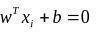
\includegraphics[width=0.8\textwidth]{assets/83}
	\caption*{}
\end{figure} (1)

\begin{figure}[H]
	\centering
	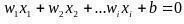
\includegraphics[width=0.8\textwidth]{assets/84}
	\caption*{}
\end{figure} (2)

\begin{figure}[H]
	\centering
	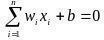
\includegraphics[width=0.8\textwidth]{assets/85}
	\caption*{}
\end{figure} \begin{figure}[H]
	\centering
	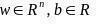
\includegraphics[width=0.8\textwidth]{assets/86}
	\caption*{}
\end{figure}
(3)

где \begin{figure}[H]
	\centering
	
\includegraphics[width=0.8\textwidth]{assets/87}
	\caption*{}
\end{figure}-- коэффициенты, определяющие все
семейство прямых, проходящих через точку
\begin{figure}[H]
	\centering
	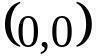
\includegraphics[width=0.8\textwidth]{assets/88}
	\caption*{}
\end{figure}. Соотношение w определяет угол линии
к осям. Ненулевой коэффициент \begin{figure}[H]
	\centering
	
\includegraphics[width=0.8\textwidth]{assets/89}
	\caption*{}
\end{figure}
позволяет линии не проходить через ноль, другими словами, это смещение.
Наклон к осям не меняется, то есть \begin{figure}[H]
	\centering
	
\includegraphics[width=0.8\textwidth]{assets/90}
	\caption*{}
\end{figure}
определяет семейство параллельных прямых,
\begin{figure}[H]
	\centering
	
\includegraphics[width=0.8\textwidth]{assets/82}
	\caption*{}
\end{figure} -- количество неизвестных переменных.
Геометрический смысл вектора \begin{figure}[H]
	\centering
	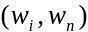
\includegraphics[width=0.8\textwidth]{assets/91}
	\caption*{}
\end{figure}
нормален к гиперплоскости {[}5{]}.

\begin{figure}[H]
	\centering
	
\includegraphics[width=0.8\textwidth]{assets/92}
	\caption*{}
\end{figure}{\bfseries -Nearest Neighbours (KNN).}
\begin{figure}[H]
	\centering
	
\includegraphics[width=0.8\textwidth]{assets/92}
	\caption*{}
\end{figure}-Nearest Neighbours (KNN) -- это тип
алгоритма машинного обучения, используемый для решения задач
классификации и регрессии. KNN основан на простой идее: объекты одного
класса обычно находятся ближе друг к другу в пространстве признаков. KNN
основан на принципе, где \begin{figure}[H]
	\centering
	
\includegraphics[width=0.8\textwidth]{assets/93}
	\caption*{}
\end{figure} обозначает
количество «ближайших соседей». Когда новый наблюдаемый случай (или
объект) требует классификации, алгоритм KNN просматривает
\begin{figure}[H]
	\centering
	
\includegraphics[width=0.8\textwidth]{assets/92}
	\caption*{}
\end{figure} ближайших соседей этого объекта из
набора обучающих данных. Затем он присваивает объекту класс, наиболее
распространенный среди этих соседей. Если
\begin{figure}[H]
	\centering
	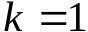
\includegraphics[width=0.8\textwidth]{assets/94}
	\caption*{}
\end{figure}, новый объект присваивается классу
его ближайшего соседа. В контексте регрессии KNN присваивает новому
объекту среднее значение \begin{figure}[H]
	\centering
	
\includegraphics[width=0.8\textwidth]{assets/92}
	\caption*{}
\end{figure} ближайших
соседей. Но раз уж мы решили взять в классификацию KNN, то не будем
особо останавливаться на регрессии. Для определения ближайших соседей
можно использовать различные метрики расстояния:

\begin{enumerate}
\def\labelenumi{\arabic{enumi}.}
\item
  Евклидовое расстояние:
\end{enumerate}

\begin{figure}[H]
	\centering
	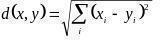
\includegraphics[width=0.8\textwidth]{assets/95}
	\caption*{}
\end{figure} (4)

\begin{enumerate}
\def\labelenumi{\arabic{enumi}.}
\setcounter{enumi}{1}
\item
  Расстояние Манхэттена:
\end{enumerate}

\begin{figure}[H]
	\centering
	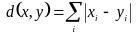
\includegraphics[width=0.8\textwidth]{assets/96}
	\caption*{}
\end{figure} (5)

\begin{enumerate}
\def\labelenumi{\arabic{enumi}.}
\setcounter{enumi}{2}
\item
  Расстояние Минковского:
\end{enumerate}

\begin{figure}[H]
	\centering
	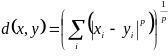
\includegraphics[width=0.8\textwidth]{assets/97}
	\caption*{}
\end{figure} (6)

где \begin{figure}[H]
	\centering
	
\includegraphics[width=0.8\textwidth]{assets/98}
	\caption*{}
\end{figure} и
\begin{figure}[H]
	\centering
	
\includegraphics[width=0.8\textwidth]{assets/99}
	\caption*{}
\end{figure} -- два экземпляра, а
\begin{figure}[H]
	\centering
	
\includegraphics[width=0.8\textwidth]{assets/100}
	\caption*{}
\end{figure}и \begin{figure}[H]
	\centering
	
\includegraphics[width=0.8\textwidth]{assets/101}
	\caption*{}
\end{figure}
-- значения признака \begin{figure}[H]
	\centering
	
\includegraphics[width=0.8\textwidth]{assets/102}
	\caption*{}
\end{figure} для
\begin{figure}[H]
	\centering
	
\includegraphics[width=0.8\textwidth]{assets/98}
	\caption*{}
\end{figure} и
\begin{figure}[H]
	\centering
	
\includegraphics[width=0.8\textwidth]{assets/99}
	\caption*{}
\end{figure}соответственно, а
\begin{figure}[H]
	\centering
	
\includegraphics[width=0.8\textwidth]{assets/103}
	\caption*{}
\end{figure} -- параметр определяющий степень
ближайших соседей.

После расчета расстояний до всех соседей в обучающей выборке KNN
выбирает \begin{figure}[H]
	\centering
	
\includegraphics[width=0.8\textwidth]{assets/92}
	\caption*{}
\end{figure} соседей, расстояние которых
минимально. Когда выбрано число \begin{figure}[H]
	\centering
	
\includegraphics[width=0.8\textwidth]{assets/92}
	\caption*{}
\end{figure} и
метрика расстояния, KNN классифицирует новые наблюдения на основе того,
какие классы наиболее распространены среди их
\begin{figure}[H]
	\centering
	
\includegraphics[width=0.8\textwidth]{assets/92}
	\caption*{}
\end{figure} ближайших соседей {[}6{]}.

{\bfseries Машины опорных векторов (SVM)}. Машины опорных векторов (SVM) --
это тип алгоритма машинного обучения, который в основном используется
для решения задач классификации, хотя его также можно применять для
регрессии и обнаружения выбросов. Целью SVM является поиск
гиперплоскости в многомерном пространстве, которая лучше всего разделяет
два класса данных {[}7{]}. Гиперплоскость -- это линия, которая делит
пространство входных объектов, создавая раздел между классами. SVM
стремится найти оптимальную гиперплоскость, которая эффективно разделяет
точки данных на основе их принадлежности к определенному классу -- это
может быть класс 0 или класс 1. Если мы представим, что это линия в
контексте двумерного пространства, разделяющая наши данные. Например:

\begin{figure}[H]
	\centering
	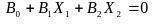
\includegraphics[width=0.8\textwidth]{assets/104}
	\caption*{}
\end{figure} (7)

где коэффициенты \begin{figure}[H]
	\centering
	
\includegraphics[width=0.8\textwidth]{assets/105}
	\caption*{}
\end{figure} и
\begin{figure}[H]
	\centering
	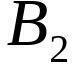
\includegraphics[width=0.8\textwidth]{assets/106}
	\caption*{}
\end{figure}, определяющие наклон линии и точку
пересечения \begin{figure}[H]
	\centering
	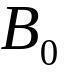
\includegraphics[width=0.8\textwidth]{assets/107}
	\caption*{}
\end{figure}, находятся с помощью
алгоритма обучения, а \begin{figure}[H]
	\centering
	
\includegraphics[width=0.8\textwidth]{assets/108}
	\caption*{}
\end{figure} и
\begin{figure}[H]
	\centering
	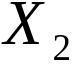
\includegraphics[width=0.8\textwidth]{assets/109}
	\caption*{}
\end{figure} -- две входные переменные.

Линия гиперплоскости позволяет проводить классификацию. Используя
уравнение линии, мы можем вставить входные значения и определить
положение новой точки относительно линии. У нас будет 4 варианта:

1) Если новая точка находится над линией, уравнение дает значение больше
нуля, и мы можем классифицировать эту точку как принадлежащую первому
классу (класс А).

2) Если новая точка находится ниже линии, уравнение дает значение меньше
нуля, и мы относим точку ко второму классу (классу B).

3) Если новая точка находится близко к линии, уравнение дает значение,
близкое к нулю, и классифицировать точку становится сложнее.

4) Если значение велико, это указывает на большую уверенность модели в
своем прогнозе.

\begin{figure}[H]
	\centering
	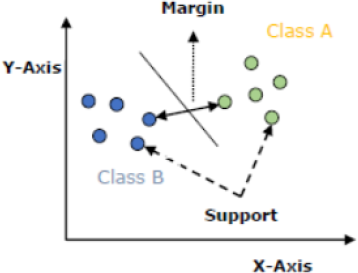
\includegraphics[width=0.8\textwidth]{assets/110}
	\caption*{}
\end{figure}

{\bfseries Рис. 1 -- Машины опорных векторов}

Расстояние между линией и ближайшими точками данных определяется как
«запас». Идеальная или оптимальная линия, которая может эффективно
разделить два класса, имеет наибольший запас. Такая линия называется
«гиперплоскостью с максимальным запасом». Запас определяется как
перпендикулярное расстояние от линии до ближайших точек. Только эти
точки важны при определении линии и создании классификатора. Такие точки
называются «опорными векторами». Они поддерживают или определяют
гиперплоскость. Гиперплоскость выбирается из обучающих данных с
использованием метода оптимизации, который максимизирует запас. На
практике данные часто хаотичны и не могут быть полностью разделены
гиперплоскостью. Из-за этого мы немного ослабляем ограничение на
максимизацию запаса в виде линии, разделяющей классы. Такой
классификатор обычно называют «классификатором с мягкими границами». Это
изменение позволяет некоторым точкам в наборе обучающих данных нарушать
границу разделительной линии {[}8{]}.

{\bfseries Случайный лес (Random Forest).} Случайный лес --- это метод
ансамблевого обучения, который объединяет несколько деревьев решений для
создания более точного и стабильного прогноза. Суть метода заключается в
построении большого количества различных деревьев решений, а затем
усреднении их прогнозов. Каждое дерево строится независимо от других.
При построении каждого дерева используются следующие случайные элементы
{[}9{]}:

1. Начальная загрузка: для построения каждого дерева из исходной выборки
данных с возвратом выбирается подвыборка. Это означает, что некоторые
экземпляры могут появляться в подвыборке более одного раза, а другие
могут вообще не появляться.

2. Подпространство случайных признаков. В каждом узле дерева решений
выборка признаков ограничивается случайным подмножеством признаков при
выборе оптимального признака для разделения.

Однако следует отметить, что при работе со Random Forest нам не нужно
обрабатывать каждое дерево отдельно. Мы просто обучаем модель на данных,
и она автоматически создает и объединяет все деревья.

\begin{figure}[H]
	\centering
	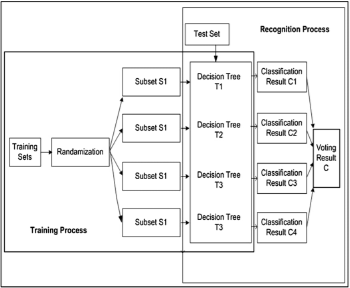
\includegraphics[width=0.8\textwidth]{assets/111}
	\caption*{}
\end{figure}

{\bfseries Рис. 2 -- Концептуальная основа классификатора случайного леса}

Существует несколько показателей, которые можно использовать для
измерения «качества» разделения в дереве решений, и эти показатели также
используются в случайном лесу {[}10{]}. Двумя наиболее распространенными
показателями являются энтропия и коэффициент Джини. Обе классификации
являются двоичными и измеряют степень «чистоты» узла.

\begin{enumerate}
\def\labelenumi{\arabic{enumi}.}
\item
  Энтропия (в случае бинарной классификации):
\end{enumerate}

\begin{figure}[H]
	\centering
	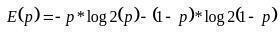
\includegraphics[width=0.8\textwidth]{assets/112}
	\caption*{}
\end{figure} (8)

\begin{enumerate}
\def\labelenumi{\arabic{enumi}.}
\setcounter{enumi}{1}
\item
  Коэффициент Джини:
\end{enumerate}

\begin{figure}[H]
	\centering
	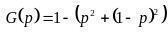
\includegraphics[width=0.8\textwidth]{assets/113}
	\caption*{}
\end{figure} (9)

где\begin{figure}[H]
	\centering
	
\includegraphics[width=0.8\textwidth]{assets/114}
	\caption*{}
\end{figure}-- вероятность того, что случайно
выбранный элемент из узла будет принадлежать классу 1. Таким образом,
если все элементы в узле принадлежат к одному классу (т.е. узел
«чистый»), энтропия и коэффициент Джини будут равны 0. Если данные
равномерно распределены между обоими классами, они достигнут
максимального значения (в случае бинарной классификации оно будет равно
0,5). В контексте случайного леса энтропия и коэффициент Джини
используются для определения наиболее эффективного разделения на каждом
этапе. Это разделение выбирается таким образом, чтобы минимизировать
взвешенную сумму энтропий или коэффициент Джини в дочерних узлах. Это
помогает создавать деревья решений, которые хорошо распределяют данные,
и приводит к более точным прогнозам по ансамблю в целом. Случайный лес в
кредитном скоринге предлагает преимущества в виде обработки большого
количества функций, устойчивости к недостающим данным и масштаба
функций, а также эффективности при работе с несбалансированными данными.
Этот алгоритм выделяет ключевые факторы при принятии кредитного решения
и снижает риск переобучения. Однако он также создает проблемы при
интерпретации результатов, требует больших вычислительных ресурсов и
может демонстрировать нестабильность прогнозирования и трудности в
прогнозировании редких событий. Также существует риск переобучения при
наличии шумовых особенностей {[}11{]}.

{\bfseries Обсуждение и результаты.} В статье использовались модели
машинного обучения, включая k-ближайшие соседи (KNN), случайный лес,
машины опорных векторов (SVM) и логистическую регрессию, а также
анализировались различные показатели. Данные были предворительно
обработаны, включая масштабирование, категориальное кодирование
признаков и удаление выбросов. Затем данные были разделены на обучающую
выборку и тестовую выборку в соотношении, обеспечивающем надежную оценку
моделей. Затем каждая модель была обучена на обучающей выборке с
использованием подходящих гиперпараметров. Далее были получены прогнозы
для тестовой выборки и сравнены с истинными значениями целевой
переменной. Результаты экспериментов показали, что все рассмотренные
модели демонстрируют ту или иную степень эффективности при решении
задачи кредитного скоринга. В частности, модели KNN, Random Forest
достигли высоких значений точности и
\begin{figure}[H]
	\centering
	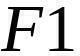
\includegraphics[width=0.8\textwidth]{assets/115}
	\caption*{}
\end{figure}-меры, что указывает на их
способность правильно классифицировать клиентов с низким и высоким
кредитным риском. С другой стороны, модели SVM и логистической регрессии
также показали приемлемые результаты, но их производительность оказалась
несколько ниже, чем у предыдущих моделей. В целом по полученным
результатам можно сделать вывод, что модели KNN, Random Forest являются
наиболее подходящими алгоритмами для задачи кредитного скоринга. Однако
этот результат может сработать не для всех наборов данных, но в нашем
конкретном случае, при работе с данными банка Хоум Кредит, они наиболее
актуальны.

Особенность кредитного скоринга заключается в том, что классифицировать
плохого заемщика как хорошего обходится дороже, чем классифицировать
хорошего заемщика как плохого. Ошибка второго рода и ошибка первого рода
соответственно; ошибка второго рода обходится кредитору гораздо дороже,
чем ошибка первого рода. В связи с этим приняты следующие метрики оценки
качества алгоритмов. Для этого введем следующие понятия {[}12{]}:

TP (True Positive) -- истинно положительный.

FP (False Positive) -- ложное срабатывание. Ошибка первого рода.

FN (False Negative) -- ложноотрицательный результат. Ошибка второго
рода.

TN (True Negative) -- истинно отрицательный.

\emph{Точность (Accuracy)} -- доля правильно классифицированных
кредитов. Самая простая метрика, но не должна быть единственной метрикой
модели, особенно когда представители разных классов встречаются с разной
вероятностью (несбалансированная выборка). Точность рассчитывается по
следующей формуле:

\begin{figure}[H]
	\centering
	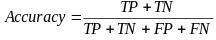
\includegraphics[width=0.8\textwidth]{assets/116}
	\caption*{}
\end{figure} (10)

\emph{Точность(Precision)} -- это доля объектов, которые классификатор
называет положительными и которые на самом деле являются положительными.
Рассчитывается по формуле:

\begin{figure}[H]
	\centering
	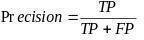
\includegraphics[width=0.8\textwidth]{assets/117}
	\caption*{}
\end{figure} (11)

\emph{Полнота(Recall)} -- доля объектов положительного класса от всех
объектов положительного класса, найденных алгоритмом. Он рассчитывается
по формуле:

\begin{figure}[H]
	\centering
	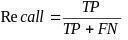
\includegraphics[width=0.8\textwidth]{assets/118}
	\caption*{}
\end{figure} (12)

\begin{figure}[H]
	\centering
	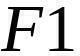
\includegraphics[width=0.8\textwidth]{assets/119}
	\caption*{}
\end{figure}оценка -- среднее гармоническое
значение точности и полноты:

\begin{figure}[H]
	\centering
	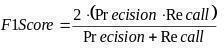
\includegraphics[width=0.8\textwidth]{assets/120}
	\caption*{}
\end{figure} (13)

Матрица путаницы -- это матричная таблица, используемая для оценки
эффективности классификатора. Обычно он указывает количество правильных
и неправильных результатов алгоритма классификации. Он также
предоставляет информацию об ошибках первого и второго порядка {[}13{]}.

{\bfseries Таблица 1 -- Матрица путаницы}

\begin{longtable}[]{@{}
  >{\raggedright\arraybackslash}p{(\columnwidth - 4\tabcolsep) * \real{0.3158}}
  >{\raggedright\arraybackslash}p{(\columnwidth - 4\tabcolsep) * \real{0.2983}}
  >{\raggedright\arraybackslash}p{(\columnwidth - 4\tabcolsep) * \real{0.3859}}@{}}
\toprule\noalign{}
\multicolumn{2}{@{}>{\raggedright\arraybackslash}p{(\columnwidth - 4\tabcolsep) * \real{0.6141} + 2\tabcolsep}}{%
\begin{minipage}[b]{\linewidth}\raggedright
Actual -- True
\end{minipage}} & \begin{minipage}[b]{\linewidth}\raggedright
\end{minipage} \\
\midrule\noalign{}
\endhead
\bottomrule\noalign{}
\endlastfoot
True Positive & False Positive(Type 1) & Predicted --
Positive/Negative \\
False Negative(Type 2) & True Negative & Predicted --
Positive/Negative \\
\end{longtable}

\begin{figure}[H]
	\centering
	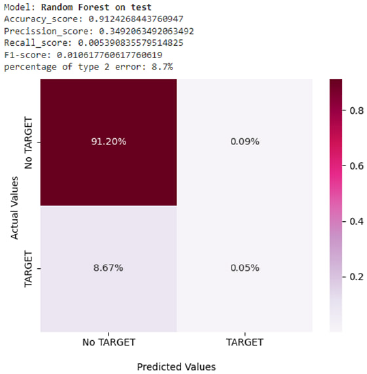
\includegraphics[width=0.8\textwidth]{assets/121}
	\caption*{}
\end{figure}

{\bfseries Рис. 3 - Результаты случайного леса}

Результаты случайного леса (Random Forest): точность - хорошая, но
увеличилось и количество ошибок второго рода. Эта модель редко
предсказывает, что человек не вернет кредит.

\begin{figure}[H]
	\centering
	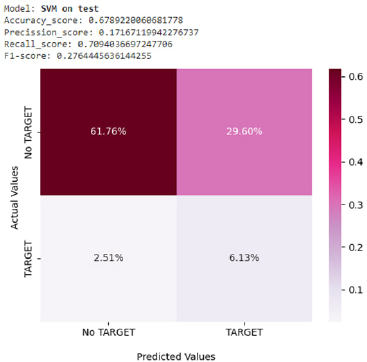
\includegraphics[width=0.8\textwidth]{assets/122}
	\caption*{}
\end{figure}

{\bfseries Рис. 4 - Результаты машины опорных векторов (SVM)}

Результаты SVM: эта модель показывает средние результаты при сравнении
логистической регрессии и случайного леса.

\begin{figure}[H]
	\centering
	\includegraphics[width=0.8\textwidth]{assets/123}
	\caption*{}
\end{figure}

{\bfseries Рис. 5- Результаты}
\begin{figure}[H]
	\centering
	\includegraphics[width=0.8\textwidth]{assets/92}
	\caption*{}
\end{figure}{\bfseries ближайщих соседей (KNN)}

\begin{figure}[H]
	\centering
	\includegraphics[width=0.8\textwidth]{assets/124}
	\caption*{}
\end{figure}

{\bfseries Рис. 6 - Результаты логистической регрессии (LR)}

Результат: из всех метрик лучше всего выделяется процент ошибок 2-го
типа, он достаточно мал, о чем свидетельствует показатель полноты.
Точность приемлемая.

{\bfseries Таблица 2 -- Результаты использованных моделей}

% \begin{longtable}[]{@{}
%   >{\raggedright\arraybackslash}p{(\columnwidth - 8\tabcolsep) * \real{0.2748}}
%   >{\raggedright\arraybackslash}p{(\columnwidth - 8\tabcolsep) * \real{0.1858}}
%   >{\raggedright\arraybackslash}p{(\columnwidth - 8\tabcolsep) * \real{0.1942}}
%   >{\raggedright\arraybackslash}p{(\columnwidth - 8\tabcolsep) * \real{0.1726}}
%   >{\raggedright\arraybackslash}p{(\columnwidth - 8\tabcolsep) * \real{0.1726}}@{}}
% \toprule\noalign{}
% \begin{minipage}[b]{\linewidth}\raggedright
% Модели
% \end{minipage} & \begin{minipage}[b]{\linewidth}\raggedright
% Accuracy
% \end{minipage} & \begin{minipage}[b]{\linewidth}\raggedright
% Precision
% \end{minipage} & \begin{minipage}[b]{\linewidth}\raggedright
% Recall
% \end{minipage} & \begin{minipage}[b]{\linewidth}\raggedright
% F1-score
% \end{minipage} \\
% \midrule\noalign{}
% \endhead
% \bottomrule\noalign{}
% \endlastfoot
% Случайный лес (Random Forest) & 0.91 & 0.35 & 0.006 & 0.01 \\
% Машины опорных векторов (SVM) & 0.68 & 0.17 & 0.71 & 0.28 \\
% \begin{figure}[H]
% 	\centering
% 	\includegraphics[width=0.8\textwidth]{assets/92}
% 	\caption*{}
% \end{figure}-Ближайших соседей (KNN) & 0.69 &
% 0.14 & 0.51 & 0.22 \\
% Логистическая регрессия & 0.7 & 0.18 & 0.68 & 0.28 \\
% \end{longtable}

{\bfseries Выводы.} В статье проведено исследование кредитного скоринга с
использованием различных машинных алгоритмов. Основной целью
исследования было создание эффективной скоринговой модели для
прогнозирования вероятности дефолта клиентов Хоум Кредит Банка. Для
достижения этой цели был использован обширный набор данных,
предоставленный Хоум Кредит Банком, содержащий информацию о клиентах и
\hspace{0pt}\hspace{0pt}их кредитной истории. Данные были предварительно
обработаны и прошли этапы очистки, масштабирования и преобразования для
подготовки к обучению модели. В исследовании применялись четыре
различных моделей машинного обучения: случайный лес, машины опорных
векторов (SVM), \begin{figure}[H]
	\centering
	\includegraphics[width=0.8\textwidth]{assets/125}
	\caption*{}
\end{figure}ближайших соседей
(KNN), логистическая регрессия. Каждая модель была обучена на обучающей
выборке и протестирована на тестовой выборке. Эксперименты позволили нам
сравнить производительность различных моделей и оценить их точность,
полноту и F1-меру на основе показателей качества классификации.
Результаты показали, что модели Random Forest, Gradient и логистической
регрессии демонстрируют наилучшую точность и полноту. Они достигают
высокой точности прогнозирования кредитного риска и принимают
эффективные решения на основе предоставленных данных. По результатам
экспериментов можно сделать следующие выводы: Модель, основанная на
ансамблевых методах, такой как Random Forest, показала лучшую
производительность среди всех протестированных моделей. Она
продемонстрировала высокую точность и стабильность в прогнозировании
кредитоспособности клиентов. Линейная модель, как логистическая
регрессия, показала низкую производительность по сравнению с другими
моделями. SVM также показала хороший результат, но немного уступали
ансамблевым моделям в точности прогнозирования. KNN оказалась наименее
эффективнымм моделям среди протестированных. Они имеют ограниченные
возможности по моделированию сложных зависимостей в данных и требуют
более тщательного подбора параметров для достижения высоких результатов.
Оценка выполнения задачи показала, что использование Random Forest
позволяет существенно повысить точность прогнозирования
кредитоспособности клиентов. Эта модель обладают способностью обобщать
данные и фиксировать сложные взаимосвязи между атрибутами, что
обеспечивает высокую точность. Пути реализации результатов исследования
могут включать следующие аспекты: финансовым организациям рекомендуется
интегрировать выбранные ансамблевые модели, такие как Random Forest,
KNN, SVM LightGBM в свою систему кредитного скоринга. Это поможет
повысить качество и достоверность прогноза погашения кредита и снизить
риск для банка.

{\bfseries Литература}

1.G.T.Balakayeva, D.K.Darkenbayev, C.Phillips. Investigation of
technologies of processing of BigData//International Journal of
Mathematics and Physics-2017.-Vol.8.- No.2.- P. 13-18.

DOI:~10.26577/ijmph.2017.v8.i2.02

2.Anderson R. The credit scoring toolkit: theory and practice for retail
credit risk management and decision automation, N.Y.: Oxford University
Press, 2007. -- 790 p. ISBN: 9780199226405

3.Lewis E.M. An introduction to credit scoring.//Athena press, 1992. --
162 p.

4.Naeem S. Credit risk scorecards: developing and implementing
intelligent credit scoring//John Wiley and Sonsю- 2015.-208 p. ISBN:
978-1-119-20173-1

5.Allison P.D. Logistic regression using the SAS system: theory and
application//Cary, NC: SAS Institute, 2001. -- 303 p. SBN:
978-0-471-22175-3

6.Mays E.(ed.) Handbook of credit scoring. Chicago: Glenlake Publishing
Company Ltd /Fitzroy Dearborn Publishers, 2001.-370 p. ISBN
978-0814406199

7.Rimmer J. Contemporary changes in credit scoring // Credit Control,
2005.-Vol.4(26)- P.56-60.

8.Rowland J. B. Confidently evaluate small businesses with credit
scoring // Business Credit, 2003.- P. 26-31.

9.G. Balakayeva, D. Darkenbayev. The solution to the problem of
processing Big Data using the example of assessing the solvency of
borrowers//Journal of Theoretical and Applied Information Technology,
2020. -- Vol. 98(3).- P 2659-2670.

10.D. Darkenbayev Big Data processing on the example of credit
scoring,//Journal of Problems in Computer Science and Information
Technologies.-2023. -Vol.1(3).- P.50-61.

DOI 10.26577/1i32jpcsit2307

11.Thomas Lyn C. A survey of credit and behavioural scoring: forecasting
financial risk of lending to consumers // International Journal of
Forecasting, 2000. -- No.16. -- Pp. 149-172.

12.Myers J.H., Forgy E.W. The development of numerical credit evaluation
systems//Journal of American Statistical
Association.-1963.-No.58.-P.799-806.

13. David W. Hosmer,~Stanley Lemeshow Applied logistic regression. -
N.-Y.: John Wiley and Sons, 2000. - P.1162-1163. DOI:10.1002/0471722146

\emph{{\bfseries Сведения об авторах}}

Даркенбаев Д.К. - PhD, и.о. доцента, Казахский национальный университет
им. аль-Фараби, Алмата, Казахстан, e-mail: dauren.kadyrovich@gmail.com;

Зиятбекова Г.З.- PhD, и.о. доцента, Казахский национальный университет
им. аль-Фараби, Алмата, Казахстан, e-mail: ziyatbekova@mail.ru;

Алтыбай А. - PhD, и.о. доцента, Казахский национальный университет им.
аль-Фараби, Алмата, Казахстан, e-mail: arshyn.altybay@gmail.com;

Мекебаев Н.О.-PhD, ассоциированный профессор, Казахский национальный
женский педагогический университет, Алматы, Казахстан, e-mail:
nurbapa@mail.ru

Жамангарин Д. С.- PhD, Казахский университет технологии и бизнеса имени
К. Кулажанова, Астана, Казахстан, е-mail: Dus\_man89@mail.ru

\emph{{\bfseries Information about the authors}}

Dauren D.-PhD, Acting Associate Professor Al-Farabi Kazakh National
University, Almaty, Kazakhstan,e-mail: dauren.kadyrovich@gmail.com;

Ziyatbekova G{\bfseries .-} PhD, Acting Associate Professor Al-Farabi
Kazakh National University, Almaty, Kazakhstan,e-mail:
ziyatbekova@mail.ru;

Altybay A.-PhD, Acting Associate Professor Al-Farabi Kazakh National
University, Almaty, Kazakhstan, e-mail: arshyn.altybay@gmail.com;

Nurbapa M.-PhD, Associate Professor of the Department of Computer
Science, Kazakh National Women\textquotesingle s Pedagogical University,
Almaty, Kazakhstan, e-mail: nurbapa@mail.ru

Zhamangarin D. S.-PhD, K. Kulazhanov Kazakh University of Technology and
Business, Astana, Kazakhstan, е-mail: Dus\_man89@mail.ru.\newpage
{\bfseries МРНТИ 50.41.29};14.01.85

{\bfseries EVALUATION OF THE EFFECTIVENESS OF USING THE SOFTWARE PRODUCT
"ASSISTANT FOR THE PREPARATION OF TEST TASKS" TO TEST THE KNOWLEDGE OF
STUDENTS}

{\bfseries \textsuperscript{1}K.Akishev\textsuperscript{🖂},\textsuperscript{1}A.Тulegulov,
\textsuperscript{1}D. Zhamangarin , \textsuperscript{1}Z.Nurtai,
\textsuperscript{2}E. Ospanov}

\textsuperscript{1}Kazakh University of Technology and Business named
after K.Kulazhanov, Astana, Kazakhstan,

\textsuperscript{2}NJSC ''Shakarim University'', Semey, Kazakhstan

{\bfseries \textsuperscript{🖂}}Correspondingauthor: Akmail04cx@mail.ru

The educational and methodological set of documentation (UMKD) is an
integral part of the educational process at a higher educational
institution.

One of the types of control of a student at a higher educational
institution is passing a test. Currently, it is the most common and
popular tool used in many disciplines, providing a transparent, fast and
quite practical way of verifying students\textquotesingle{} knowledge.

When developing tests, teachers use various programs, while spending
quite a lot of time to prepare, first, control questions, and then add
them to the appropriate program.

In this regard, the purpose of our research is the need to develop
software code that allows you to use ChatGPT for the automated formation
of test tasks when checking the knowledge of students.

The developed computer program "Assistant for the preparation of test
tasks" allows you to automate the process of preparing test tasks for
text of any volume and number of questions;

The program code can be used in educational institutions of the Ministry
of Education and the Ministry of Science and Higher Education of the
Republic of Kazakhstan.

The practical application of the developed program "Assistant for the
preparation of test tasks" allows to increase the effectiveness of the
teacher\textquotesingle s work by 80\% compared to existing analogues
for the development of test tasks. At the same time, the quality and
adequacy of the developed issues are at a high level.

{\bfseries Key words}: automation, information technology, software
product, test tasks, efficiency, student.

{\bfseries БІЛІМ АЛУШЫЛАРДЫҢ БІЛІМІН ТЕКСЕРУ ҮШІН "ТЕСТ ТАПСЫРМАЛАРЫН
ДАЙЫНДАУ КӨМЕКШІСІ" БАҒДАРЛАМАЛЫҚ ӨНІМІН ПАЙДАЛАНУ}

{\bfseries ТИІМДІЛІГІН БАҒАЛАУ}

{\bfseries \textsuperscript{1}К.Акишев\textsuperscript{🖂},
\textsuperscript{1}А.Тулегулов, \textsuperscript{1}Д. Жамангарин,
\textsuperscript{1}Ж.Нұртай, \textsuperscript{2}Е.Oспанов}

\textsuperscript{1}Қ.Құлажанов атындағыҚазақ технология және бизнес
университеті АҚ, Астана, Казахстан ,

\textsuperscript{2}Шакарим атындағы университет КЕАҚ, Семей, Қазақстан,

е-mail:Akmail04cx@mail.ru

Құжаттаманың оқу-әдістемелік жиынтығы (ОӘК) жоғары оқу орнындағы оқу
процесінің ажырамас бөлігі болып табылады.

Жоғары оқу орнында білім алушыны бақылаудың бір түрі-тест тапсыру.
Қазіргі уақытта бұл көптеген пәндер бойынша қолданылатын ең кең таралған
және танымал құрал, білім алушылардың білімін тексерудің мөлдір, жылдам
және практикалық түрін қамтамасыз етеді.

Тесттерді әзірлеу кезінде мұғалімдер әртүрлі бағдарламаларды
пайдаланады, ал алдымен тест сұрақтарын дайындауға, содан кейін оларды
тиісті бағдарламаға енгізуге жеткілікті уақыт ресурстары жұмсалады.

Осыған байланысты, біздің зерттеуіміздің мақсаты білім алушылардың
білімін тексеру кезінде тест тапсырмаларын автоматтандырылған
қалыптастыру үшін chatgpt пайдалануға мүмкіндік беретін бағдарламалық
кодты әзірлеу қажеттілігі болып табылады.

"Тест тапсырмаларын дайындау көмекшісі" компьютеріне арналған әзірленген
бағдарлама тест тапсырмаларын дайындау процесін автоматтандыруға
мүмкіндік береді, кез-келген көлемдегі мәтін мен сұрақтар саны үшін;

Бағдарламалық код Қазақстан Республикасы Білім министрлігі мен ғылым
және жоғары білім министрлігінің Білім беру мекемелерінде пайдаланылуы
мүмкін.

Әзірленген "тест тапсырмаларын дайындау көмекшісі" бағдарламасын
практикалық қолдану тест тапсырмаларын әзірлеу үшін қолданыстағы
аналогтармен салыстырғанда оқытушының жұмыс тиімділігін 80\% - ға
арттыруға мүмкіндік береді. Бұл ретте әзірленген мәселелердің сапасы мен
барабарлығы жоғары деңгейде.

{\bfseries Түйін сөздер}: автоматтандыру, ақпараттық технологиялар,
бағдарламалық өнім, тест тапсырмалары, тиімділік, білім алушы

{\bfseries ОЦЕНКА ЭФФЕКТИВНОСТИ ИСПОЛЬЗОВАНИЯ ПРОГРАММНОГО ПРОДУКТА
«ПОМОЩНИК ПОДГОТОВКИ ТЕСТОВЫХ ЗАДАНИЙ» ДЛЯ ПРОВЕРКИ ЗНАНИЙ ОБУЧАЮЩИХСЯ}

{\bfseries \textsuperscript{1}К.Акишев\textsuperscript{🖂},
\textsuperscript{1}А.Тулегулов, \textsuperscript{1}D.Zamangarin,
\textsuperscript{1}Ж. Нуртай, \textsuperscript{2}Е.Oспанов}

\textsuperscript{1}Казахский университет технологии и бизнеса
им.К.Кулажанова, Астана, Казахстан,

\textsuperscript{2} НАО Университет Шакарима, Семей,Казахстан,

е-mail: Akmail04cx@mail.ru

Учебно-методический комплект документации (УМКД), является неотъемлемой
частью учебного процесса в высшем учебном заведении.

Одним из видов контроля обучающегося в высшем учебном заведении является
прохождение теста. В настоящее время --это наиболее распространенный и
популярный инструмент? используемый по многим дисциплинам,
обеспечивающий, прозрачный, быстрый и довольно практичный вид проверки
знаний обучающихся.

При разработке тестов преподаватели используют различные программы, при
этом тратится довольно большой ресурс времени, чтобы подготовить,
сначала контрольные вопросы, а затем внести их в соответствующую
программу.

В этой связи, цель нашего исследования заключается в необходимости
разработки программного кода позволяющего, использовать ChatGPT, для
автоматизированного формирования тестовых заданий, при проверки знаний
обучающихся.

Разработанная программа для ЭВМ «Помощник подготовки тестовых заданий»
позволяет автоматизировать процесс подготовки тестовых заданий, для
текста любого объема и количества вопросов;

Программный код может быть использован в образовательных учреждениях
министерства образования и министерства науки и высшего образования
Республики Казахстан.

Практическое применение разработанной программы «Помощник подготовки
тестовых заданий» позволяет повысить эффективность работы преподавателя
на 80\% по сравнению с существующими аналогами для разработки тестовых
заданий. При этом качество и адекватность разработанных тестовых
вопросов на высоком уровне.

{\bfseries Ключевые слова}: автоматизация, информационные технологии,
программный продукт, тестовые задания, эффективность, обучающийся

{\bfseries Introduction.} The adoption of the Law on Digitalization in the
Republic of Kazakhstan {[}1{]} requires the use of information
technology achievements in all sectors of the economy, including in the
field of education {[}2{]}.

It should be understood that the effectiveness of obtaining high-quality
education ensures objective control of students\textquotesingle{}
knowledge and skills. In practice, two types of control are used --
subjective and objective. The first one is characterized by the personal
ideas of the examiner in relation to the student. And in practice, it
may not always be objective, for a number of reasons, including the
teacher\textquotesingle s likes and dislikes for the student. As for the
second type of control, which is now used both in schools and in higher
educational institutions, they include a criterion-oriented test, which
serves as a measure of the quality of learning by students.

If we ask ourselves why testing has become so widely used, then we get
the answer:

1) a more adequate and reliable method that allows students to be put on
an equal footing;

2) mobilizes the work of the brain in conditions of maximum
concentration and responsibility;

3) Excludes human influence.

One of the main criteria of software products used for test control is
saving time, as well as time spent on developing software code.

Although the material costs associated with the use of testing are much
higher from the point of view of the organization, but the efficiency is
much higher.

Table 1 shows the most common test development programs.

{\bfseries Table 1−Test development programs}

\begin{longtable}[]{@{}
  >{\raggedright\arraybackslash}p{(\columnwidth - 2\tabcolsep) * \real{0.3137}}
  >{\raggedright\arraybackslash}p{(\columnwidth - 2\tabcolsep) * \real{0.6863}}@{}}
\toprule\noalign{}
\begin{minipage}[b]{\linewidth}\raggedright
Title
\end{minipage} & \begin{minipage}[b]{\linewidth}\raggedright
Functional
\end{minipage} \\
\midrule\noalign{}
\endhead
\bottomrule\noalign{}
\endlastfoot
TestMaker & -editing previously created tests;

-save test results;

-adding graphic images;

-Generate questions in random order. \\
RichTest & Differs from the previous one by the possibility of:

-transition to theory to prepare for the test;

- setting the difficulty of each question;

- attaching a hint to a question

- the user switches to the training mode. \\
Экзаменатор & Practically no different from TestMaker \\
MyTestXPro & The difference from the previous ones:

-single selection;

-multiple choice;

-establishment of the order of succession;

-establishing compliance;

-indication of the truth or falsity of statements; \\
INDIGO & Features:

-tasks for each group of individual settings. \\
\end{longtable}

The disadvantages of the above programs are the need for manual
formation of questions, considerable time for the development of tests.

In this regard, there is a problem in the need to automate the
preparation of test tasks while maintaining the quality of the
questions, the ability to edit, the availability of adequate ergonomics
and use for mobile applications.

The purpose of the study: The development of software code that allows
you to automate the process of preparing test tasks using ChatGPT
capabilities.

{\bfseries Materials and methods.} The computer program "Assistant for
preparing test tasks" was developed using JavaScript, HTML, CSS to
create HTTP requests and interact with the ChatGPT API.

{\bfseries Discussion of the results.} The development of the program code
begins with going to the project folder and http://localhost:3000 we
will launch the development server.

{\bfseries Open the file located at the address (see fig.1)}

\begin{figure}[H]
	\centering
	\includegraphics[width=0.8\textwidth]{assets/126}
	\caption*{}
\end{figure}

{\bfseries Figure 1− Index.html files}

Our React application will be placed in the \textless div
id="root"\textgreater{} line. The element will be replaced with the
application code, and everything else will remain the same.

Open the src / index js file, the React application is located here, the
source code of the application is located in the src directory (see fig.
2).

Let\textquotesingle s look at the code of our first component. Src / App
(see fig. 3).

\begin{figure}[H]
	\centering
	\includegraphics[width=0.8\textwidth]{assets/127}
	\caption*{}
\end{figure}

{\bfseries Figure 2−Index.js files}

\begin{figure}[H]
	\centering
	\includegraphics[width=0.8\textwidth]{assets/128}
	\caption*{}
\end{figure}

{\bfseries Figure 3− App.js files}

Let\textquotesingle s consider the principle of using ChatGPT in our
study.

By creating HTTP API requests, we can interact with ChatGPT and receive
responses in real time {[}3-8{]}.

This requires tools and accounts in particular:

-\/-Open ID account and API key (registering an account on the Open AI
platform and obtaining an API key to authenticate ChatGPT API requests;

-the presence of a Node.js and npm;

-a project in the React JS Project.

The next important point is to create a component to control the chat
function (see listing 1 of the program code).The program is written
using the Russian alphabet.

Listing 1 of the program code:

// Chat.js

Import React , \{ useState \} внутринний
\textquotesingle react\textquotesingle{} ;

аксиомы \textquotesingle axios\textquotesingle{} внутрениий импорт;

const чат = () =\textgreater{} \{

const {[}input, setInput{]} = useState
(\textquotesingle\textquotesingle);

const {[}известия, setMessages{]} = useState({[}{]});

const sendMessage = async() =\textgreater{} \{

он бір

if (вход. Trim () === \textquotesingle\textquotesingle) возвращение;

// ChatGPT API-ге выполните запрос

попытка \{

const ответ = аксиома ожидание. почты (

\textquotesingle https://api.openai.com/v1/engines/davinci-codex/completions\textquotesingle{}
,

\{

определение: ввод,

максимальное\_символов: 150,

\},

\{

темы: \{

"Тип контента ": "application/json"

\textquotesingle Авторизация\textquotesingle{} : \textquotesingle Media
\$\{ процесс . конв. REACT\_APP\_OPENAI\_API\_KEY \}`

\},

\}

);

// Обновите Статус, используя ответ

тридцать

setMessages ({[} ... сообщение , \{ текст : ввод , тип :
\textquotesingle пользователь\textquotesingle{} \}{]});

setMessages ({[} ... сообщение , \{ текст : ответ .выбор данных {[} 0
{]}. текст , тип: \textquotesingle месяц\textquotesingle{} \}{]});

setInput(\textquotesingle\textquotesingle);

\} catch (ошибка) \{

консоль error(\textquotesingle\textquotesingle Ошибка отправки сообщения
:\textquotesingle, ошибка);

\}

\};

выход (

\textless ситуация \textgreater{}

\textless ситуация \textgreater{}

\{Карта сообщений(( сообщение , индекс ) =\textgreater{} (

\textless div ключ = \{индекс\} className = \{сообщение. \}
\textgreater введите

\{ информация . тип \}

\textless/del\textgreater{}

))\}

\textless/del\textgreater{}

\textless случай\textgreater{}

\textless тип ввода = «тип»

мән = \{ввод\}

onChange = \{( e ) =\textgreater{} setInput ( например. задача .
значение )\}

Заполните = "Введите сообщение..."

/\textgreater{}

\textless{} button onClick = \{ sendMessage \}
\textgreater Отправить\textless/button\textgreater\hspace{0pt}

\textless/del\textgreater{}

\textless/del\textgreater{}

);

\};

Open AI Chatbot API Node.js provides developers with a framework for
creating intelligent interactive web applications {[}9-12{]}.

Let\textquotesingle s consider a request to the server and create a
download verification component and consider all this using React Hooks.

Let\textquotesingle s create a new React: os create-rect-top
rect-axios-table project.

Follow the link: cd react-axios-table

We use an array of objects as data for our project (see listing 2 of the
program code).

Listing 2 of the program code:

{[}

\{

id: 101,

firstName: \textquotesingle Sue\textquotesingle,

lastName: \textquotesingle Corson\textquotesingle,

email: \textquotesingle DWhalley@in.gov\textquotesingle,

phone: \textquotesingle(612)211-6296\textquotesingle,

address: \{

streetAddress: \textquotesingle9792 Mattis Ct\textquotesingle,

city: \textquotesingle Waukesha\textquotesingle,

state: \textquotesingle WI\textquotesingle,

zip: \textquotesingle22178\textquotesingle{}

\},

description: \textquotesingle et lacus magna dolor...\textquotesingle,

\}

{]}

Importing axioms into a component that sends requests to the server:
import axios from \textquotesingle axis\textquotesingle{} in the project
we use React Hooks, useState and import useEffect.

Adding the following code to the component: function App() \{ (see
listing 3 of the program code).

Listing 3 of the program code:

const {[}appState, setAppState{]} = useState();

useEffect(() =\textgreater{} \{

const apiUrl =
\textquotesingle http://www.filltext.com/?rows=32\&id=\{number\textbar1000\}\&firstName=\{firstName\}\&lastName=\{lastName\}\&email=\{email\}\&phone=\{phone\textbar(xxx)xxx-xx-xx\}\&address=\{addressObject\}\&description=\{lorem\textbar32\}\textquotesingle;

axios.get(apiUrl).then((resp) =\textgreater{} \{

const allPersons = resp.data;

setAppState(allPersons);

\});

\}, {[}setAppState{]});

return (

\textless div className="app"\textgreater{}

\textless/div\textgreater{}

);

\}

export default App;

The above code checks isLoading when data is loaded and shows a loading
message, if isLoading is erroneous, it is returned.

Let\textquotesingle s consider the description of the program code
"Assistant for preparing test tasks". Fig. 4 shows the entrance to the
program {[}13{]}.

\begin{figure}[H]
	\centering
	\includegraphics[width=0.8\textwidth]{assets/129}
	\caption*{}
\end{figure}

{\bfseries Figure 4−Login to the program}

The user can log in as a teacher with admin rights, or as a student fig.
5;6.

\begin{figure}[H]
	\centering
	\includegraphics[width=0.8\textwidth]{assets/130}
	\caption*{}
\end{figure}

{\bfseries Figure 5−Entering the program as a teacher}

\begin{figure}[H]
	\centering
	\includegraphics[width=0.8\textwidth]{assets/131}
	\caption*{}
\end{figure}

{\bfseries Figure 6−Entering the program as a student}

The presented software product on the main page contains educational
programs in the disciplines for which it is supposed to develop tests
fig.7.

\begin{figure}[H]
	\centering
	\includegraphics[width=0.8\textwidth]{assets/132}
	\caption*{}
\end{figure}

{\bfseries Figure 7−The main menu of the program code "Assistant for
preparing test tasks"}

Each educational program contains disciplines in which the student is
tested fig.8.

\begin{figure}[H]
	\centering
	\includegraphics[width=0.8\textwidth]{assets/133}
	\caption*{}
\end{figure}

{\bfseries Figure 8−An example of disciplines for testing students}

The development of tests begins with entering the name of the discipline
(in our example, the subject "Controller Programming" for the
educational program is Automation and control), the number of test
questions, and the time to answer fig.9.

\begin{figure}[H]
	\centering
	\includegraphics[width=0.8\textwidth]{assets/134}
	\caption*{}
\end{figure}

{\bfseries Figure 9−Development of test tasks}

The user (teacher) enters the number of questions and the time to answer
manually. The material for the tests can be prepared in advance or
obtained from the Internet, a textbook, a synopsis, etc. sources. After
entering the text into the window, the "create test" button is pressed
Fig.9. A few minutes are enough to create a test using ChatGPT for a
large number of questions. In our test task (see fig. 8) 25 questions
and 20 minutes to answer. We can see the result in fig. 10-11.

\begin{figure}[H]
	\centering
	\includegraphics[width=0.8\textwidth]{assets/135}
	\caption*{}
\end{figure}

{\bfseries Figure 10− Developed test questions from 1-6}

\begin{figure}[H]
	\centering
	\includegraphics[width=0.8\textwidth]{assets/136}
	\caption*{}
\end{figure}

{\bfseries Figure 11− Developed test questions from 20-25}

The resulting test is automatically placed in the Educational Programs
automation and Management folder fig.12.

\begin{figure}[H]
	\centering
	\includegraphics[width=0.8\textwidth]{assets/137}
	\caption*{}
\end{figure}

{\bfseries Figure 12- Developed test on the discipline "Controller
programming"}

Students of the groups are added to the appropriate discipline to
complete the test tasks fig.13, this requires their login and email in
gmail.com.

\begin{figure}[H]
	\centering
	\includegraphics[width=0.8\textwidth]{assets/138}
	\caption*{}
\end{figure}

{\bfseries Figure 13−Adding students to control knowledge}

After the registration of a student, he can take a test to check his
knowledge of the disciplines of the educational program in accordance
with the curriculum.

Fig. 14 shows the answer to the test tasks in the discipline "Controller
programming".

\begin{figure}[H]
	\centering
	\includegraphics[width=0.8\textwidth]{assets/139}
	\caption*{}
\end{figure}

{\bfseries Figure 14- Completing the answers to the test}

The result of the response can be viewed in a separate folder fig.15.

\begin{figure}[H]
	\centering
	\includegraphics[width=0.8\textwidth]{assets/140}
	\caption*{}
\end{figure}

{\bfseries Figure 15−Storage location for students\textquotesingle{}
answers}

The result of the answer is given as a percentage of the equivalent
number of points received by students fig.16.

\begin{figure}[H]
	\centering
	\includegraphics[width=0.8\textwidth]{assets/141}
	\caption*{}
\end{figure}

{\bfseries Figure 16−The result of the student\textquotesingle s answer to
the test questions}

Currently, the program code does not generate graphical tasks, and it
does not have the possibility of randomization, since these tasks were
not set for research purposes.

{\bfseries Conclusion.} The developed computer program "Assistant for the
preparation of test tasks" allows you to automate the process of
preparing test tasks for text of any volume and number of questions;

The program code can be used in educational institutions of the Ministry
of Education and the Ministry of Science and Higher Education of the
Republic of Kazakhstan and does not require high-performance computers
and a large amount of memory.

The practical application of the developed program "Assistant for the
preparation of test tasks" allows to increase the effectiveness of the
teacher\textquotesingle s work by 80\% compared to existing analogues
for the development of test tasks. At the same time, the quality and
adequacy of the developed issues are at a high level.

{\bfseries Referenses}

1. Zakon Respubliki Kazakhstan. O vnesenii izmenenii I dopolnenii v
netkotorie zakonodatel'nie akti Respubliki Kazakhstan po voprosam
stimulirovaniya innovacii, razvitiya cifrovizacii, informacionnoi
bezopasnosti i obrazovaniya. Rasporyazhenie Prem'er ministra RK ot 25
avgusta 2022 goda № 128-r. URL:https://online.zakon.kz/ Document/
?doc\_id=33516174. {[}in Russ.{]}

2.Nestik T.A. ,Zhuravlev A.L. Social'no psikhologicheskaya determinaciya
gotovnostilichnosti k ispolzovaniu novikh tekhnologii
{[}Socio-psychological determination of a person\textquotesingle s
readiness to use new technologies// Psychological Journal.-
2018.-Т.39(5). -С. 5-14.

DOI 10.31857/S020595920000829-7 {[}in Russ.{]}

3.Brazdil, P., Jorge, A. Progress in Artificial Intelligence: Knowledge
Extraction, Multi-Agent Systems, Logic Programming, and Constraint
Solving; Springer: Berlin/Heidelberg, Germany, 2001.-418P. ISBN
9783540430308

4.M. Montenegro-Rueda{\bfseries ,}J. Fernández-Cerero{\bfseries ,}José M.
Fernández-Batanero, E. López-Meneses. Impact of the Implementation of
ChatGPT in Education: A Systematic Review.//Computers.-\emph{~}2023.-
Vol.12(8).- P. 153.-P.1-13. ~DOI 10.3390/computers12080153

5.García-Peña, V.R.; Mora-Marcillo, A.B.; Ávila-Ramírez, J.A. La
inteligencia artificial en la educación// Domino De Las Cienc.
-2020.-Vol. 6 (3).- P. 648-666. DOI 10.23857/dc.v6i3.1421

6. Incio Flores, F.A., Capuñay Sánchez, D.L., Estela Urbina, R.O.,
Valles Coral, M.A., Vergara Medrano, S.E.,EleraGonzáles, D.G.
Inteligencia artificial eneducación: Unarevisión de la literatura en
revistas científicas internacionales// Revista de Investigación Apuntes
Universitarios. - ~2022.-Vol. 12(1)- P.353-372. DOI
10.17162/au.v12i1.974

7. Neuman, M.; Rauschenberger, M.; Schön, E.M. We Need To Talk About
ChatGPT: The Future of AI and Higher Education//Hochschule
Hannover.-2023.- P.1-4. DOI 10.25968/opus-2467

8. García Sánchez, O.V. Uso y Percepción de ChatGPTen la Educación
Superior// RITI Journal

-2023.- Vol. 11(23).- P.98-107. DOI 10.36825/RITI.11.23.009

9. Osorio, J.A.C. Explorando el potencial de ChatGPTen la
escrituracientífica: Ventajas, desafíos y precauciones// Sci. Et
Tech.-2023.-Vol.28(01).- P.3-5.DOI 10.22517/23447214.25303

10. Qadir, J. Engineering Education in the Era of ChatGPT: Promises and
Pitfalls of Generative AI for Education//IEEE Global Engineering
Education Conference (EDUCON).- 2023.

DOI 10.1109/EDUCON54358.2023.10125121

11. Wang T., Lund B.D., Marengo A., Pagano A., Mannuru N.R., Teel Z.A.,
Pange J. Exploring the Potential Impact of ArtificialIntelligence (AI)
on International Students in Higher Education: Generative AI, Chatbots,
Analytics, and International Student Success// Appl.Sci -2023. -Vol. 13,
6716. DOI 10.20944/preprints202305.0808.v1

12. García-Peñalvo, F.J. La percepción de la Inteligencia Artificial
encontextoseducativostras el lanzamiento de ChatGPT: Disrupcióno pánico
// Educ. Knowl. Soc. (EKS). -2023.-Vol 24, e31279. DOI
10.14201/eks.31279

13 Аkishev K. Computer program "Assistant for the preparation of test
tasks. Certificate of entry of information into the State register of
rights to copyrighted objects No. 48275 dated July 10, 2024. NIISRK.

\emph{{\bfseries Informationabouttheauthors}}

Akishev K. M. - Candidate of Technical Sciences, Ass. Professor, Kazakh
University of Technology and Business named after K. Kulazhanov, Astana,
Kazakhstan, e -mail:akmail04cx@mail.ru;

Tulegulov A. D.- Candidate of physics and mathematics Sciences, Ass.
Professor, Kazakh University of Technology and Business named after. K.
Kulazhanov,Astana, Kazakhstan,e-mail:tud62@yandex.ru;

Zhamangarin D. S.- Ph.D., Ass. Professor, Kazakh University of
Technology and Business named after. K. Kulazhanov, Astana, Kazakhstan
e-mail:dus\_man89@mail.ru;

Nurtai Z.T. - Ph.D., Ass. Professor, Kazakh University of Technology and
Business named after. K. Kulazhanov,Astana, Kazakhstan, e-mail:
zhadira\_nurtai@mail.ru;

Ospanov E. А.- PhD, Associate Professor,NAO Shakarim University, Semey,
Kazakhstan, e -mail:78oea@mail.ru;

\emph{{\bfseries Информация об авторах}}

Акишев К. М. -к.т.н., асс. профессор, Казахский университет технологии и
бизнеса им. К. Кулажанова,Астана, Казахстан,e-mail:akmail04cx@mail.ru;

Тулегулов А. Д.- к.ф.м.н., асс. профессор, Казахский университет
технологии и бизнеса им. К. Кулажанова,Астана, Казахстан:
e-mail:tud62@yandex.ru;

Жамангарин Д. С.- доктор PhD , асс. профессор Казахский университет
технологии и бизнеса им. К. Кулажанова, Астана,
Казахстан,e-mail:dus\_man89@mail.ru;

Нуртай Ж.Т. - доктор PhD, асс. профессор, Казахский университет
технологии и бизнеса им. К. Кулажанова,

Астана, Казахстан, e-mail: zhadira\_nurtai@mail.ru;

Оспанов Е. А.- доктор PhD, асс. профессор, НАО «Университет имени
Шакарима, Семей, Казахстан, e-mail:78oea@mail.ru\newpage
{\bfseries МРНТИ 20.23.15}

{\bfseries ТАБИҒИ ТІЛДЕ ПАЙДАЛАНУШЫ ИНТЕРФЕЙСТЕРІН ҚҰРУ ӘДІСТЕРІ}

{\bfseries \textsuperscript{1}А.Ж. Танирбергенов, \textsuperscript{1}С.К.
Серикбаева\textsuperscript{🖂}, \textsuperscript{2}Б.У. Бөбеева,
\textsuperscript{3}Ш.Е. Ахметжанова,}

{\bfseries \textsuperscript{3}А.Д. Абдувалова}

\textsuperscript{1}Л.Н.Гумилев атындағы Еуразия ұлттық университеті,
Астана қ., Қазақстан,

\textsuperscript{2}Орталық Азия Инновациялық Университеті, Шымкент,
Қазақстан,

\textsuperscript{3}М.Х.Дулати атындағы Тараз өңірлік университеті, Тараз
қ., Қазақстан

Корреспондент-автор: inf\_8585@mail.ru

Қазіргі заманғы технологиялық даму жағдайында пайдаланушы интерфейстері
адамның компьютерлік бағдарламалармен немесе құрылғылармен өзара
әрекеттесуінде маңызды рөл атқарады, бұл олардың қарапайымдылығы,
тиімділігі және жалпы пайдаланушы тәжірибесін анықтайды. NLP UI идеясы
табиғи тілді өңдеу (NLP), машиналық оқыту және жасанды интеллект
алгоритмдерін қолдануға негізделген. Зерттеу барысында осындай
интерфейстерді құру әдістері, олардың артықшылықтары мен шектеулері,
сонымен қатар оларды одан әрі дамыту перспективалары талқыланды. ТТИ
платформаларын талдау, мысалы, Google Dialogflow, Microsoft Bot
Framework, Wit.ai, IBM Watson Assistant және Amazon Lex, пайдаланушыға
ыңғайлы интерфейстерді дамытуда маңызды рөл атқарады. Әдістер мен
материалдар бөлімінде табиғи тілде пайдаланушы интерфейстерін жасауға
арналған қолданыстағы әдістер, соның ішінде сөйлеуді тану және синтездеу
жүйелері, машиналық оқыту алгоритмдері және морфологиялық, синтаксистік
және семантикалық талдау талқыланады. Бұл тәсілдер пайдаланушы
сұраныстарын тереңірек түсінуге және дәлірек жауаптар беруге мүмкіндік
береді.

{\bfseries Түйінді сөздер:} табиғи тіл, интерфейс, табиғи тілді өңдеу
(NLP), семантика, сұраныс.

{\bfseries МЕТОДЫ СОЗДАНИЯ ПОЛЬЗОВАТЕЛЬСКИХ ИНТЕРФЕЙСОВ НА ЕСТЕСТВЕННОМ
ЯЗЫКЕ}

{\bfseries \textsuperscript{1}А.Ж. Танирбергенов, \textsuperscript{1}С.К.
Серикбаева\textsuperscript{🖂}, \textsuperscript{2}Б.У. Бөбеева,
\textsuperscript{3}Ш.Е. Ахметжанова,}

{\bfseries \textsuperscript{3}А.Д. Абдувалова}

\textsuperscript{1}Евразийский национальный университет имени
Л.Н.Гумилева, Астана, Казахстан \textsuperscript{2}Центрально-Азиатский
инновационный университет, Шымкент, Казахстан

\textsuperscript{3}Таразский региональный университет им.М. Х. Дулати,
Тараз, Казахстан

e-mail:inf\_8585@mail.ru

В данной работе рассматриваются методы и технологии создания
пользовательских интерфейсов на естественном языке. В условиях
современного технологического развития пользовательские интерфейсы
играют важную роль во взаимодействии человека с компьютерными
программами и устройствами, что определяет их простоту, эффективность и
общий пользовательский опыт. Идея пользовательского интерфейса на основе
NLP основана на использовании алгоритмов обработки естественного языка
(NLP), машинного обучения и искусственного интеллекта. В ходе
исследования обсуждались методы создания таких интерфейсов, их
преимущества и ограничения, а также перспективы дальнейшего развития.
Анализ платформ TTI, таких как Google Dialogflow, Microsoft Bot
Framework, Wit.ai, IBM Watson Assistant и Amazon Lex, показал их важную
роль в разработке удобных интерфейсов. В разделе "Методы и материалы"
обсуждаются существующие методы создания пользовательских интерфейсов на
естественном языке, включая системы распознавания и синтеза речи,
алгоритмы машинного обучения, а также морфологический, синтаксический и
семантический анализ. Эти подходы позволяют глубже понять запросы
пользователей и давать более точные ответы.

{\bfseries Ключевые слова:} естественный язык, интерфейс, обработка
естественного языка (NLP), семантика, запрос.

{\bfseries METHODS FOR CREATING USER INTERFACES IN NATURAL LANGUAGE}

{\bfseries \textsuperscript{1}А. Tanirbergenov, \textsuperscript{1}S.
Serikbayeva\textsuperscript{🖂}, \textsuperscript{2}B. Bobeeva,
\textsuperscript{3}Sh. Akhmetzhanova,}

{\bfseries \textsuperscript{3}A. Abduvalova}

\textsuperscript{1}L.N. Gumilyov Eurasian National University,Department
of Information Systems, Astana, Kazakhstan

Central Asian Innovation University, Shymkent, Kazakhstan

\textsuperscript{3}Taraz Regional University named after M.KH.Dulaty,
Taraz, Kazakhstan

e-mail: inf\_8585@mail.ru

This paper discusses methods and technologies for creating user
interfaces in natural language. In the context of modern technological
development, user interfaces play an important role in human interaction
with computer programs and devices, which determines their simplicity,
efficiency and overall user experience. The idea of an NLP-based user
interface is based on the use of natural language processing (NLP)
algorithms, machine learning and artificial intelligence. The research
discussed methods for creating such interfaces, their advantages and
limitations, as well as prospects for further development. Analysis of
TTI platforms such as Google Dialogflow, Microsoft Bot Framework, Wit.ai
, IBM Watson Assistant and Amazon Lex, showed their important role in
the development of user-friendly interfaces. The Methods and Materials
section discusses existing methods for creating user interfaces in
natural language, including speech recognition and synthesis systems,
machine learning algorithms, as well as morphological, syntactic and
semantic analysis. These approaches allow for a deeper understanding of
user requests and provide more accurate answers.

{\bfseries Keywords:} natural language, interface, natural language
processing (NLP), semantics, query.

{\bfseries Кіріспе.} Технологияны дамытудың қазіргі әлемінде пайдаланушы
интерфейстері адамның компьютерлік бағдарламамен немесе құрылғымен өзара
әрекеттесуінде шешуші рөл атқарады. Олар пайдаланудың қарапайымдылығын,
жұмыс тиімділігін және жалпы пайдаланушы тәжірибесін анықтайды. Осы
саладағы елеулі жетістіктерге қарамастан, ыңғайлы және интуитивті
пайдаланушы интерфейстерін құру әзірлеушілер үшін қиын болып қала
береді.

Бұл мәселені шешудің инновациялық тәсілдерінің бірі-табиғи тілде
пайдаланушы интерфейстерін құру әдісі (natural language UI, NLP UI). Бұл
әдіс пайдаланушыларға басқа адаммен сөйлесу сияқты табиғи тілді қолдана
отырып, бағдарламалық жасақтамамен немесе құрылғымен өзара әрекеттесуге
мүмкіндік береді. Бұл тәсіл интуитивті және икемді өзара әрекеттесудің
жаңа мүмкіндіктерін ашады.

Табиғи тілде пайдаланушы интерфейстерін құру идеясы табиғи тілді өңдеу
алгоритмдерін (Natural Language Processing, NLP), машиналық оқытуды және
жасанды интеллектті қолдануға негізделген. Бұл технологиялар жүйелерге
табиғи тілді түсінуге және түсіндіруге, сондай-ақ тиісті жауаптар мен
командаларды құруға мүмкіндік береді {[}1{]}.

NLP UI артықшылықтары айқын: бұл құрылғылар мен бағдарламалық
жасақтаманың өзара әрекеттесуін пайдаланушылар үшін табиғи және
интуитивті етеді, бұл оқу уақытын қысқартады және пайдалану тиімділігін
арттырады. Осының арқасында пайдаланушылар жаңа өнімдер мен қызметтерді
тезірек игере алады, сонымен қатар күнделікті тапсырмаларды тиімдірек
орындай алады.

Дегенмен, оның артықшылықтарына қарамастан, табиғи тілде пайдаланушы
интерфейстерін жасау да өзінің қиындықтары мен шектеулеріне тап болады.
Олардың бірі-пайдаланушы сұраныстарын дәл түсінудің қиындығы, әсіресе
тілдің түсініксіз немесе күрделі конструкциялары жағдайында.

Дегенмен, технологияның дамуымен және жаңа NLP әдістері мен
алгоритмдерінің пайда болуымен бұл мәселелер біртіндеп азайып, табиғи
тілдегі пайдаланушы интерфейстерін барған сайын танымал және қолжетімді
етеді. Бұл зерттеуде біз осындай интерфейстерді құрудың әртүрлі
әдістерін, олардың артықшылықтары мен шектеулерін және оларды одан әрі
дамыту перспективаларын қарастырамыз.

Табиғи тілдік интерфейстерді (ТТИ) құру платформаларын талдау табиғи
тілді өңдеу саласын дамытудағы маңызды қадам болып табылады (Natural
Language Processing, NLP). Бұл платформалар әзірлеушілерге техникалық
мәліметтерді терең түсінбестен мәтін мен сөйлеуді өңдеу мүмкіндіктерін
қолданбалар мен қызметтерге біріктіруге мүмкіндік береді.

Бірінші назар аударарлық платформа - Google-дің Dialogflow. Ол
чатботтарды, виртуалды көмекшілерді және басқа да ТТИ -ді құрудың кең
функционалдығын ұсынады. Dialogflow мәтінді талдаудың, интенттер мен
контекстті анықтаудың және басқа Google қызметтерімен интеграциялаудың
қуатты құралдарына ие {[}2{]}.

Тағы бір маңызды платформа-Microsoft Bot Framework. Бұл мәтіндік ғана
емес, сонымен қатар дауыстық интерфейстерді де қолдайтын чат-боттарды
әзірлеуге арналған құралдар жиынтығы. Azure интеграциясының арқасында
Bot Framework Машиналық оқыту модельдерінің ауқымдылығы мен оқу
мүмкіндіктерін ұсынады.

Wit.ai Facebook-тен-ТТИ -ді дамытуға арналған тағы бір танымал
платформа. Ол қолданудың қарапайымдылығымен және әртүрлі тілдерді жақсы
қолдауымен танымал. Wit.ai мәтін мен аудионы өңдеуге арналған API,
сондай-ақ өз модельдеріңізді құруға және үйретуге арналған құралдарды
ұсынады.

IBM Watson Assistant-бұл ТТИ құрудың тағы бір қуатты құралы. Ол интентті
тану, мәтіннің тоналдылығын талдау және әртүрлі байланыс арналарымен
интегрциялау сияқты көптеген мүмкіндіктерді ұсынады. Watson Assistant
сонымен қатар көмекшілерді масштабтау және жекелендіру мүмкіндіктерін
ұсынады.

Amazon Lex-Amazon Web Services компаниясының табиғи тілді өңдеу қызметі.
Ол сөйлеуді тану және синтездеу мүмкіндіктерін, сондай-ақ басқа AWS
қызметтерімен интеграцияны қамтамасыз етеді. Amazon Lex дайын модельдер
мен машиналық оқыту құралдарын қолдана отырып, жоғары деңгейлі ТТИ
құруға мүмкіндік береді.

Табиғи тілде пайдаланушы интерфейстерін құруда адам мен компьютерлік
жүйенің тиімді өзара әрекеттесуін анықтайтын іргелі теориялық принциптер
бар. Бұл принциптерге лингвистикалық негіздер, өзара әрекеттесу
психологиясы, интерфейс дизайны, табиғи тілді өңдеу технологиялары
(NLP), Машиналық оқыту және интерфейс психологиясы кіреді.

Лингвистикалық принциптер сәйкес сөздер мен сөз тіркестерін таңдауға,
мәтінді құрылымдауға және пайдаланушылардың сұраныстарын дұрыс
түсіндіруге мүмкіндік береді. Өзара әрекеттесу психологиясы ақпаратты
қабылдау, шешім қабылдау және кері байланысқа жауап беру ерекшеліктерін
ескеруге көмектеседі. Интерфейс дизайны ыңғайлы және тартымды
интерфейстерді құруға ықпал ететін ақпараттың визуалды ұйымдастырылуын
анықтайды {[}3{]}.

Табиғи тілді өңдеу технологиялары (NLP) табиғи тілдегі мәтінді талдауды,
түсінуді және генерациялауды қамтамасыз етуде маңызды рөл атқарады.
Машиналық оқыту және жасанды интеллект интерфейстерге пайдаланушы
тәжірибесі негізінде жұмысын жақсартуға мүмкіндік береді. Интерфейс
психологиясы адамдардың интерфейстермен қалай әрекеттесетінін түсінуге
көмектеседі және оларды оңтайландыру принциптерін ұсынады. Осы теориялық
негіздердің барлығы пайдаланушылардың қажеттіліктеріне сәйкес келетін
және пайдаланудың ыңғайлылығы мен тиімділігін қамтамасыз ететін табиғи
тілде пайдаланушы интерфейстерін құруды қамтамасыз ету арқылы өзара
әрекеттеседі.

Іс жүзінде осы теориялық принциптерді қолдану кешенді тәсілді және нақты
жағдайды мұқият талдауды қажет етеді. Бұл талдау мақсатты аудиторияның
ерекшеліктерін, олардың қажеттіліктерін, жүйені пайдалану мәнмәтінін,
сондай-ақ техникалық шектеулер мен мүмкіндіктерді зерттеуді
қамтиды.Келесі қадам-интерфейстің прототиптерін жасау және
пайдаланушылардың қатысуымен тестілеу. Бұл пайдаланушылардың нақты
қажеттіліктері мен қалауларын ескере отырып, кері байланыс алуға және
интерфейстің дизайны мен функционалдығына түзетулер енгізуге мүмкіндік
береді. Алынған кері байланыс пен пайдалану ортасындағы өзгерістер
негізінде интерфейсті үнемі жетілдіру және жаңарту оның өзектілігі мен
тиімділігін сақтаудың негізгі аспектісі болып табылады {[}4{]}.
Осылайша, табиғи тілде пайдаланушы интерфейстерін құрудың теориялық
негіздері пайдаланушы тәжірибесін жақсартуға және мақсаттарға жетуге
ықпал ететін ыңғайлы, интуитивті және тиімді жүйелерді әзірлеу бойынша
практикалық жұмыстың негізін құрайды.

Пайдаланушы интерфейстеріндегі табиғи тіл ұғымы адам мен компьютерлік
жүйенің өзара әрекеттесуінің ыңғайлылығы мен тиімділігін қамтамасыз
етуде шешуші рөл атқарады. Бұл контекстегі табиғи тіл пайдаланушылардың
өз ойлары мен сұрауларын арнайы командаларды немесе техникалық
терминдерді үйренуді қажет етпестен, әдеттегі әңгімедегідей жеткізе білу
қабілетін білдіреді. Табиғи тілді пайдалану техникалық дайындық
деңгейіне қарамастан, пайдаланушылардың кең ауқымы үшін интуитивті
интерфейстер жасауға мүмкіндік береді. Мұндай интерфейстер табиғи және
ыңғайлы өзара әрекеттесуді қамтамасыз етеді, кіру шегін азайтады және
оқу процесін жылдамдатады.

Пайдаланушы интерфейстерінде табиғи тілді қолданудың бір мысалы-Apple,
Google Assistant және Amazon Alexa Siri сияқты виртуалды көмекшілер. Бұл
жүйелер пайдаланушыларға табиғи тілді қолдана отырып, сұрақтар қоюға
және дауыспен командалар беруге мүмкіндік береді, бұл өзара әрекеттесу
процесін табиғи және ыңғайлы етеді.

Пайдаланушы интерфейстерінде табиғи тіл ұғымын одан әрі дамыту Машиналық
оқыту және табиғи тілді өңдеу (Natural Language Processing, NLP)
технологияларымен интеграцияны қамтиды. Бұл жүйелерге сұраныстардың
мәнмәтінін түсінуге, тілдің нюанстарын ескеруге және тіпті
пайдаланушылардың кері байланысы негізінде қабілеттерін жақсартуға
мүмкіндік береді.

Қазіргі заманғы қосымшалар мен құрылғыларда табиғи тілді талдау
негізінде жұмыс істейтін автотолтыру және автоматты түзету функциялары
жиі кездеседі. Бұл теруді жылдам әрі ыңғайлы етеді, қателіктер
ықтималдығын азайтады.

Табиғи тіл сонымен қатар Ақылды үйді басқаруға арналған интерфейстер
саласында маңызды рөл атқарады, мұнда пайдаланушылар өз құрылғыларын
табиғи тілдегі қарапайым командаларды қолдана отырып басқара алады, бұл
өмірді ыңғайлы және тиімді етеді.

Бұл тұжырымдаманың болашақ дамуы сөйлеуді тану мен контекстті түсінудің
одан да жетілдірілген технологияларын қамтуы мүмкін, бұл пайдаланушы
интерфейстеріндегі адам мен компьютерлік жүйе арасындағы одан да табиғи
және икемді өзара әрекеттесуге әкеледі.

Пайдаланушы интерфейстеріндегі табиғи тіл (Natural Language in User
Interfaces) -- бұл пайдаланушыға орыс немесе ағылшын сияқты қарапайым
адам тілін қолдана отырып, компьютерлік жүйемен немесе қосымшамен өзара
әрекеттесу мүмкіндігін беру тәсілі. Бұл интерфейсті түсінікті, қол
жетімді және пайдаланушыларға ыңғайлы етеді, өйткені олар белгілі бір
командаларды немесе интерфейс элементтерін есте сақтаудың қажеті жоқ.

Пайдаланушы интерфейстерінде табиғи тілді қолдану сөйлеуді тану және
синтездеу функцияларын, мәтінді өңдеуді, семантиканы талдауды және т.б.
қамтуы мүмкін {[}5{]}. Бұл пайдаланушыларға жүйе автоматты түрде
түсіндіретін және өңдейтін өз тілін пайдаланып сұрақтар қоюға,
командалар беруге немесе ақпарат сұрауға мүмкіндік береді.

Бұл тәсіл құрылғылармен және қосымшалармен өзара әрекеттесуді едәуір
жеңілдетеді, әсіресе техникалық интерфейстермен тәжірибесі жоқ немесе
белгілі бір командаларды үйренуге уақыт жұмсағысы келмейтін
пайдаланушылар үшін. Сондықтан әзірлеушілер ыңғайлы және интуитивті
пайдаланушы интерфейстерін жасау үшін әртүрлі табиғи тіл технологияларын
белсенді түрде зерттейді және енгізеді.

Пайдаланушы интерфейстеріндегі табиғи тілдің көптеген артықшылықтары
бар. Ең бастысы-интерфейстің қол жетімділігі мен ыңғайлылығын жақсарту
{[}6{]}. Пайдаланушыларға құрылғымен немесе қосымшамен өзара әрекеттесу
оңайырақ және ыңғайлы болады, өйткені олар күрделі командаларды немесе
интерфейс функционалдығын есте сақтаудың қажеті жоқ.

Сонымен қатар, табиғи тілді қолдану интуитивті және жекелендірілген
өзара әрекеттесуге мүмкіндік береді. Пайдаланушылар өздерінің
сұраныстары мен тілектерін табиғи стильде білдіре алады, бұл пайдалану
тәжірибесін жағымды және тиімді етеді.

Табиғи тілді өңдеу технологиялары үнемі дамып келеді және күн өткен
сайын дәлірек және жетілдіріліп отырады. Бұл Пайдаланушының тілін
түсініп қана қоймай, оның қалауы мен мінез-құлқына бейімделе алатын
ақылды интерфейстерді құрудың жаңа мүмкіндіктерін ашады.

Тұтастай алғанда, пайдаланушы интерфейстерінде табиғи тілді пайдалану
технологияны пайдаланушылардың барлық санаттары үшін мейірімді және
қолжетімді етуге көмектеседі, бұл әртүрлі құрылғылар мен қолданбалардың
қанағаттану деңгейі мен тиімділігіне ықпал етеді.

{\bfseries Материалдар мен әдістер.} Табиғи тілде пайдаланушы
интерфейстерін жасау (Natural Language User Interfaces, NLU) қазіргі
ақпараттық технологиялар әлемінде барған сайын танымал бола түсуде. Бұл
компьютерлік жүйелермен өзара әрекеттесудің ыңғайлы және интуитивті
тәсілдеріне қажеттіліктің артуына байланысты. Осы саладағы қолданыстағы
әдістер мен технологияларды шолу қазіргі даму жағдайын және одан әрі
даму бағыттарын түсінуге мүмкіндік береді.

Табиғи тілде пайдаланушы интерфейстерін құрудың негізгі әдістерінің бірі
табиғи тілді өңдеу (NLP) технологияларын пайдалану болып табылады. Бұл
технологиялар компьютерлерге табиғи тілді түсінуге және талдауға
мүмкіндік береді, олар пайдаланушылармен адамдар сияқты әрекеттесе
алатын интерфейстер жасауға мүмкіндік береді {[}7{]}.

Қолданыстағы әдістер мен технологиялардың ішінде пайдаланушыларға
дауыстық командалар мен сұраныстарды пайдалана отырып, компьютермен
өзара әрекеттесуге мүмкіндік беретін сөйлеуді тану және синтездеу
жүйелері ерекшеленеді. Мұндай жүйелер пайдаланушыларға ыңғайлы болу үшін
дауыстық көмекшілерде, мобильді құрылғыларда және басқа қолданбаларда
белсенді қолданылады.

Табиғи тілдегі пайдаланушы интерфейстерін құрудың тағы бір маңызды
аспектісі машиналық оқыту алгоритмдерін әзірлеу және пайдалану болып
табылады. Бұл алгоритмдер интерфейстерді тиімдірек және пайдалануды
жеңілдете отырып, пайдаланушының әртүрлі байланыс мәнерлері мен
сипаттамаларына бейімделе алатын үлгілерді жасауға мүмкіндік береді.

Табиғи тілде пайдаланушы интерфейстерін құру саласындағы елеулі
жетістіктерге қарамастан, одан әрі зерттеу мен дамытуды талап ететін
көптеген қиындықтар мен мәселелер әлі де бар {[}8{]}. Оларға сөйлеуді
тану дәлдігін жақсарту, контекстті түсінуді жақсарту және компьютерлік
жүйелермен бай қарым-қатынас жасау үшін басқа технологиялармен біріктіру
кіреді.

Интерфейс пайдаланушының өзара әрекеттесуінің ыңғайлылығы мен
тиімділігін қамтамасыз етуге арналған кез келген бағдарламалық жүйенің
ажырамас бөлігі болып табылады. Ол соңғы пайдаланушыға бағытталған және
бағдарлама туралы жалпы әсерді қалыптастыруда негізгі рөл атқарады.
Көбінесе пайдаланушы интерфейстің ыңғайлылығы мен анықтығына негізделген
қолданбаны пайдалануды шешеді.

Интерфейсті әзірлеу -- пайдаланушының қажеттіліктерін мұқият талдауды
және түсінуді талап ететін күрделі және көп уақытты қажет ететін
процесс. Сарапшылардың пікірінше, интерфейсті жобалау және әзірлеу
жобаны жүзеге асыруға кететін уақыттың жартысынан көбін құрайды {[}9{]}.

Интерфейстің функционалдық аспектілерін ғана емес, сонымен қатар оның
эстетикалық дизайнын, визуалды әсерін және ыңғайлылығын да ескеру
маңызды. Идеал интерфейс интуитивті, шарлау оңай және мақсатты
аудиторияның қажеттіліктерін қанағаттандыруы керек. Бағдарламаның әсері
және оның нарықта сәтті жүзеге асуы пайдаланушы интерфейсінің қаншалықты
жақсы құрастырылғанына байланысты.

Пайдаланушы интерфейсін анықтаудың бірнеше негізгі жолдары бар:

1. Тіл спецификациясы: Бұл жағдайда интерфейстің синтаксисін анықтау
үшін арнайы тілдер қолданылады. Бұл тілдер декларативті, объектіге
бағытталған, оқиғаға негізделген және т.б.

2. Графикалық спецификация: визуалды бағдарламалау, демонстрациялар және
үлгілер арқылы интерфейсті анықтаумен айналысады. Бұл әдіс әдетте
интерфейстердің шектеулі жиынтығын қолдайды.

3. Объектіге бағытталған тәсілге негізделген спецификация: Объектілерді
тікелей манипуляциялау принципіне негізделген. Пайдаланушы өңдеушілер,
мәзірлер, диалогтық терезелер және түймелер сияқты жеке нысандармен
әрекеттеседі.

4. Қолданбалы тапсырманың семантикасына негізделген интерфейс
спецификациясы: Интерфейс қолданбалы тапсырманың семантикасының
спецификациясы негізінде автоматты түрде жасалады. Дегенмен, интерфейсті
сипаттаудың күрделілігі дамуды бәсеңдетуі мүмкін.

Бүгінгі күні оларды жүзеге асырудың әртүрлі әдістерін қолдайтын
интерфейстерді әзірлеуге арналған көптеген құралдар бар {[}10{]}. Олар
бар үлгілер мен параметрленген құрамдастарды пайдалану арқылы жаңа
интерфейстерді жасауды жеңілдетеді.

Графикалық пайдаланушы интерфейстерін жылдам және сапалы әзірлеуге
арналған ең кең тараған пакет Motif болып табылады. Солтүстік Американың
OSF консорциумында әзірленген бұл пакет Xt Intrinsics идеяларының дамуы
болып табылады.

Табиғи тілді өңдеудің әртүрлі тәсілдері бар. Алғашқы тәсілдердің бірі
сөйлемге синтаксистік талдау жасауға негізделген. Бұл кезеңде сөйлем
ішіндегі синтаксистік байланыстар анықталып, сөйлемнің түрі, құрылымы
анықталады. Ол үшін талданатын тілге байланысты арнайы лексикалық және
синтаксистік ережелер қолданылады.

Сөйлемді талдау процесі тізбектей және бірнеше кезеңмен жүзеге
асырылады. Ол морфологиялық және морфемиялық талдау кезеңдерін
қадағалайды. Бұл кезеңде әрбір сөздің басқа сөйлем мүшелерімен байланысы
алынады, бұл грамматикалық категориялардың мағыналарын анықтауға
мүмкіндік береді.

Морфологиялық талдау синтаксистік талдаудың алдында тұрады және әрбір
сөздің сөйлем мүшесі, септелуі, регистр және басқалары сияқты
морфологиялық белгілерін анықтауға мүмкіндік береді. Бұл белгілер
сөйлемнің синтаксистік құрылымын анықтауда шешуші рөл атқарады {[}11{]}.

Морфологиялық сипаттамалардың саны мен әртүрлілігі нақты тілге
байланысты өзгеруі мүмкін, бұл талдау процесіне де әсер етеді.

Орыс тіліндегі табиғи тілді морфологиялық талдау үшін әртүрлі тәсілдер,
соның ішінде ықтималдық көзқарас, «бұлдыр» және «қытырлақ» морфология
қолданылады. Дегенмен, бұл процесте ең көп таралған тәсіл «айқын»
морфологияны қолдануға негізделген.

«Айқын» тәсіл орыс сөздерінің негізгі флекстік формаларын және олардың
сәйкес кодтарын қамтитын «Зализняк» сөздігі сияқты грамматикалық
сөздікке сүйенеді. Бұл сөздік ережелерге негізделген сөздің барлық
мүмкін формаларын көрсетуге мүмкіндік береді. Морфологиялық талдау
талданатын сөздің морфологиялық белгілерін анықтау үшін осы сөз
формалары мен олардың кодтарын пайдаланады.

Зализняктың грамматикалық сөздігіне негізделген сөздікті құру процесі
әрқайсысы үшін сөз формаларының жиынтығы жасалған барлық сөздерді
санаудан басталады. Бұл сөз формалары кейіннен морфологиялық талдауда
қолдану үшін сөздікке енгізіледі. Осылайша, бұл сөздік талданатын сөздің
морфологиялық сипаттамасын береді {[}12{]}.

Бұл табиғи тілді өңдеу әдісі сөздердің морфологиялық ерекшеліктерін дәл
анықтауға мүмкіндік береді, бұл орыс тіліндегі мәтіндерді талдау кезінде
маңызды қадам болып табылады.

Орыс тілінің морфемиялық талдауы әрбір сөзді префикс, жалғау, түбір,
жұрнақ және түбір сияқты құрамдас бөліктерге бөлуге мүмкіндік береді.
Бұл сөздің құрылымын және оның грамматикалық ерекшеліктерін түсінуге
көмектесетін мәтінді өңдеудің маңызды кезеңі.

Дегенмен, орыс тіліндегі морфемалардың сөздігі, әдетте, сөзде қандай
морфемалар бар екендігі туралы ақпарат береді, бірақ әрбір морфеманың
түрін көрсетпейді. Мысалы, сөздің қай бөлігі префикс, қайсысы түбір
екенін көрсетпейді. Бұл сөздің құрылымын морфемалық сөздіктегі
мәліметтерге сүйене отырып, біржақты анықтауға болмайтынын білдіреді
{[}13{]}.

Бұл ретте орыс сөзіндегі морфемалар тізбегі әдетте қатаң түрде
анықталады. Сөз префикстен, содан кейін түбірден басталып, жұрнақ пен
жалғаумен аяқталады. Алайда бұл бөліктердің кейбірі сөзде жоқ болуы
мүмкін.

Морфемалық сөздікте жоқ сөзді талдау үшін орыс тіліндегі морфемалардың
стандартты тізбегін, сондай-ақ мағыналарының ауыспалылығымен шектелетін
мүмкін префикстер, жұрнақтар және жалғаулардың тізімін пайдалануға
болады. Бұл сөзді талдауға және морфемалық сөздіктегі анық мәліметтерсіз
де оның құрылымын анықтауға мүмкіндік береді.

Сонымен, орыс тілінің морфематикалық талдауы құрылымды түсінудің маңызды
құралы болып табылады.

Табиғи тілдегі пайдаланушы сұранысын өңдеу әдісінің шамамен диаграммасы:

1. Морфологиялық талдау:

- Сұрауды жеке сөздерге талдау.

- Әр сөздің сөйлем мүшесі, септелуі, регистр және басқалары сияқты
морфологиялық белгілерін анықтау.

2. Талдау:

\begin{itemize}
\item
  Сөйлемдегі сөздер арасындағы синтаксистік байланыстарды анықтау.
\item
  Сөйлемнің бас және басыңқы мүшелерін анықтау.
\item
  Ұсыныс түрін анықтау.
\end{itemize}

3. Семантикалық талдау:

- Сұраныстың мағынасын және оның мазмұнын талдау.

- Өтініште көрсетілген мақсаттар мен міндеттерді анықтау.

- Сұранысты оның мағыналық мағынасын ескере отырып түсіндіру.

Семантикалық талдау кезеңі сөйлемнің құрылымын және оның жеке сөздерінің
мағынасын түсінуге ғана емес, мәтін элементтері арасындағы мағыналық
байланыстарды анықтай отырып, оның мақсат-міндеттер контекстіндегі
сұранысты түсінуге мүмкіндік береді {[}14{]}.

Талдаудың барлық үш кезеңін бірге пайдалану пайдаланушы сұрауын
тереңірек және толық түсінуге мүмкіндік береді, бұл өз кезегінде
ақпаратты дәлірек және тиімді өңдеуге және пайдаланушыға сәйкес жауап
немесе нәтиже беруге көмектеседі.

Семантикаға негізделген табиғи тілдегі сұрауды өңдеу әдісі мәтінді
талдаудың бірнеше кезеңдерін қамтиды. Бірінші кезең -- морфологиялық
талдау -- сөзді префикс, түбір, жұрнақ және жалғау сияқты құрамдас
бөліктеріне талдаудан тұрады. Одан кейін синтаксистік талдау
жүргізіледі, мұнда сөздер мен сөйлем құрылымы арасындағы байланыстар
анықталады. Дегенмен, тек талдау әдісінің кемшілігі - сұраудың мағынасын
түсінбеу.

Бұл мәселені шешу үшін семантикалық талдау кіреді. Бұл кезеңде өтініштің
мәні мен оның маңыздылығы түсініледі. Сонымен, табиғи тілдік сұранысты
өңдеу әдісі келесі кезеңдерді қамтиды: морфологиялық, синтаксистік және
семантикалық талдау.

Бұл әдістің диаграммасы осы кезеңдердің ретін көрсетеді, мұнда әрбір
келесі кезең алдыңғысының нәтижелері бойынша құрылады. Бұл тәсіл
пайдаланушы сұранысын тереңірек түсінуді және мәтінді дәлірек өңдеуді
қамтамасыз етеді (1-сурет).

\begin{figure}[H]
	\centering
	\includegraphics[width=0.8\textwidth]{assets/142}
	\caption*{}
\end{figure}

{\bfseries 1 -- сурет. Семантика негізінде табиғи тілдегі сұранысты өңдеу
әдісінің схемасы}

Семантикаға негізделген табиғи тілдің сұранысын өңдеу әдісінің схемасы -
табиғи тілдегі қолданушылардың сұраныстарын олардың мағыналық мазмұнын
ескере отырып түсінуге арналған кешенді тәсіл. Бұл әдіс сөйлемнің
грамматикалық құрылымын ғана емес, оның семантикасын, яғни сөздердің
мағыналары мен байланыстарын талдауға негізделген.

Сұранысты өңдеу процесінің басында лексикалық талдау жүргізіледі, оның
барысында мәтін жеке лексемаларға немесе сөздерге бөлінеді. Содан кейін
морфологиялық талдау жүргізіледі, оның нәтижесінде әрбір лексемаға
өзіндік морфологиялық форма беріледі, бұл олардың сөйлеу бөлігін және
грамматикалық сипаттамаларын анықтауға мүмкіндік береді.

Келесі кезекте синтаксистік талдау жүргізіледі, оның барысында сөйлемнің
құрылымы мен оның сөздер арасындағы синтаксистік тәуелділіктері
анықталады. Бұл сұраныстың негізгі құрамдас бөліктерін және олардың
өзара байланысын түсінуге мүмкіндік береді. Бұл ретте сұраныс
контекстіндегі сөздер мен сөз тіркестерінің мағынасы мен мағынасын
анықтауға бағытталған семантикалық талдау орын алады {[}15{]}.

Сұрау мағынасын және оның білім қорымен немесе контекстпен байланысын
тереңірек түсіну үшін машиналық оқыту әдістері мен әдістерін және
жасанды интеллектті қолдануды қамтитын семантикалық өңдеу жүргізіледі.
Бұл семантикалық модельдерді құруды, сөздердің векторлық бейнелерін және
семантикалық графиктерді немесе онтологияларды пайдалануды қамтуы
мүмкін.

Ақырында, талдау мен өңдеудің барлық кезеңдерінен кейін жауап жасалады
немесе сұраныстың түсінілген мағынасына сәйкес тиісті әрекеттер
орындалады. Бұл ақпарат үшін дерекқорды іздеуді, қолданбаларда немесе
жүйелерде операцияларды орындауды немесе пайдаланушы сұрауына табиғи
тілде жауап жасауды қамтуы мүмкін.

Іздеу сұранысын өңдеу логикасындағы негізгі диаграммалар мен
диаграммалар тиімді ақпаратты іздеу жүйелерін жобалаудың негізгі
құралдары болып табылады. Олар сұранысты өңдеу процесін
визуализациялауға және іздеу жүйелерінің логикасын түсінуге көмектеседі.
Негізгі схемалардың бірі сұранысты талдау, сәйкес деректерді іздеу және
нәтижелерді пайдаланушыға ұсыну кезеңдерін қамтитын сұранысты өңдеу
схемасы болып табылады {[}16{]}. Тағы бір маңызды схема - оңай қол
жеткізу және іздеу үшін деректерді ұйымдастыру жолдарын анықтайтын
индекстеу схемасы. Мәліметтер ағынының диаграммалары мен күй
диаграммалары сұранысты өңдеу процесін және жүйе құрамдастарының өзара
әрекетін көрсету үшін де қолданылады. Бұл диаграммалар мен диаграммалар
бірге іздеу жүйелерінің қалай жұмыс істейтіні туралы түсінік береді және
әзірлеушілерге олардың өнімділігі мен функционалдығын оңтайландыруға
көмектеседі (2-сурет).

Ақпаратты іздеу сұрауының реттілігі диаграммасы ақпаратты іздеу сұрауы
кезінде орын алатын әрекеттер тізбегін көрсетеді. Әдетте пайдаланушының
қолданба немесе веб-сайт интерфейсі арқылы сұрауды бастауымен басталады.

\begin{figure}[H]
	\centering
	\includegraphics[width=0.8\textwidth]{assets/143}
	\caption*{}
\end{figure}

{\bfseries 2 -- сурет. Ақпаратты іздеу сұранысын өңдеуге арналған реттілік
диаграммасы}

Содан кейін жүйе бұл сұрауды алады және сұранысты сәйкес іздеу жүйесіне
немесе дерекқорға жіберу арқылы іздеу процесін бастайды. Осыдан кейін
іздеу жүйесі сұрауды талдайды, сәйкес деректерді таңдайды және оны
пайдаланушыға көрсету үшін жүйеге қайтарады. Содан кейін жүйе алынған
нәтижелерді пайдаланушы ақпаратты көре және талдай алатын интерфейс
арқылы пайдаланушыға көрсетеді. Соңында, пайдаланушы сұрауды нақтылау
немесе қосымша зерттеу үшін нақты нәтижені таңдау сияқты берілген
нәтижелерге негізделген қосымша әрекеттерді жасай алады.

Қолданба интеграциясы - алынған ақпаратты қолданба ішінде шешім қабылдау
немесе Пайдаланушымен өзара әрекеттесу үшін пайдалануға болады. Мысалы,
жүйе пайдаланушының сұрағына жауап бере алады, мәтінді іздей алады
немесе мәтіндік хабарламаның көңіл-күйін талдай алады (3-сурет).

\begin{figure}[H]
	\centering
	\includegraphics[width=0.8\textwidth]{assets/144}
	\caption*{}
\end{figure}

{\bfseries 3 -- сурет. Табиғи тілді өңдеу схемасы}

Табиғи тілді өңдеу коды:

\emph{doc = nlp(transcript)}

\emph{lemmatized\_stemmed\_text = {[}stemmer.stem(token.lemma\_.lower())
for token in doc if token.is\_alpha and not token.is\_stop{]}}

Ақпарат үшін дерекқорды іздеу және клиентке жауап беру туралы сөз
болғанда, тиімді және дәл нәтиже алу үшін белгілі бір қадамдарды орындау
маңызды. Ең алдымен, іздеу критерийлері мен сұраныстың негізгі
параметрлерін анықтау қажет. Бұл нақты іздеу үшін қажетті кілт сөздерді,
күндерді, деректер түрлерін немесе басқа сипаттарды қамтуы мүмкін.

Шарттар анықталғаннан кейін дерекқорды сәйкес құралдар немесе сұрау тілі
арқылы іздеу керек. Дұрыс сұрау синтаксисін және іздеу үшін кестелер мен
өрістерді дұрыс таңдауды ескеру маңызды. Сұрау орындалғаннан кейін
дерекқор сәйкес нәтижелерді қайтарады, содан кейін оларды өңдеу
керек.Алынған деректерді өңдеу клиенттің немесе соңғы пайдаланушының
талаптарына сәйкес ақпаратты талдауды және сүзуді қамтиды. Бұл
сұрыптауды, топтастыруды, есептеулерді және қажетті жауапқа жету үшін
басқа деректерді өңдеуді қамтуы мүмкін. Деректерді өңдегеннен кейін
жауап құрылады, ол құрылымдалған және клиент үшін түсінікті болуы керек.

Маңызды қадам клиентке оны бермес бұрын алынған жауаптың дұрыстығы мен
толықтығын тексеру болып табылады. Бұл деректердің дұрыстығын және
жауаптың көрсетілген критерийлер мен талаптарға сәйкестігін тексеруді
қамтиды. Қажет болған жағдайда ақпаратты нақтылау үшін қосымша
тексерулер мен талдаулар жүргізілуі мүмкін.

Тексеруден кейін жауап клиентке беруге дайын. Бұл мәтіндік хабарлама,
есеп, кесте немесе клиентке қолдануға ыңғайлы басқа пішім түрінде болуы
мүмкін. Ұсынылған жауаптың клиенттің үмітіне сай болуын және оның
сұрауын толық қанағаттандыруын қамтамасыз ету маңызды.

Тиімді іздеуді және клиентке жауап беруді қамтамасыз ету үшін
дерекқордың жаңартылып, жаңартылып тұруын қамтамасыз ету де маңызды. Бұл
нақты іздеу нәтижелерін қамтамасыз ету үшін деректерді үнемі жаңартуды,
жаңа жазбаларды қосуды және ескірген деректерді жоюды қамтиды.

Сонымен қатар, деректердің қауіпсіздігін қамтамасыз ету және деректер
базасына қол жеткізу ережелерін сақтау қажет. Бұған пайдаланушылар үшін
сәйкес кіру құқықтарын орнату және рұқсатсыз кіруді немесе деректерге
өзгертулерді болдырмау үшін деректер әрекетін бақылау кіреді.

Жалпы алғанда, мәліметтер базасын тиімді іздеу және клиентке жауап беру
үшін іздеу критерийлерін анықтау, сұранысты орындау, деректерді өңдеу,
жауаптың дұрыстығын тексеру және оны клиентке ұсыну сияқты жүйелі тәсіл
қажет. Осы қадамдарды орындау ақпараттың клиенттерге дәл және уақтылы
берілуін қамтамасыз етуге көмектеседі (4-сурет).

1. Өңделген таңбалауыштардың массиві табиғи тілде өңдеуден кейін келеді.
Массив толық мәтінді іздеу арқылы дерекқорды іздеуге жіберіледі.

\emph{search\_results = collection.find( \{
\textquotesingle\$text\textquotesingle:
\{\textquotesingle\$search\textquotesingle: \textquotesingle{}
\textquotesingle.join(lemmatized\_stemmed\_text)\} \},
\{\textquotesingle score\textquotesingle:
\{\textquotesingle\$meta\textquotesingle:
\textquotesingle textScore\textquotesingle\},
\textquotesingle workTopic\textquotesingle: 1, "жұмыс атауы":1,\})}

2. Толық мәтінді іздеу нәтижелері курсор ретінде қайтарылады.
Деректермен жұмыс істеудің ыңғайлы нұсқасы үшін түрлендіру әрбір нысан
әрбір жазба туралы деректерді сақтайтын нысандар массивіне жасалады.

\emph{search\_results\_list =
list(search\_results.sort({[}(\textquotesingle score\textquotesingle,
pymongo.DESCENDING){]}))}

3. Іздеу нәтижелері дәл болу үшін табылған объектілерді сүзгілеу
жүргізіледі. Ол үшін жұмыс атауы және жұмыс тақырыбы өрістерін өңдеу
табиғи тілде орындалады.

\emph{for result in search\_results\_list: work\_topic =
result.get(\textquotesingle workTopic\textquotesingle,
\textquotesingle\textquotesingle) \# Получаем значение поля workTopic
work\_name = result.get(\textquotesingle workName\textquotesingle,
\textquotesingle\textquotesingle) \# Получаем значение поля workName \#
Применяем стемминг, лемматизацию и приведение к нижнему регистру
lemmatized\_stemmed\_topic = {[}stemmer.stem(token.lemma\_.lower()) for
token in nlp(work\_topic) if token.is\_alpha and not token.is\_stop{]}
lemmatized\_stemmed\_name = {[}stemmer.stem(token.lemma\_.lower()) for
token in nlp(work\_name) if token.is\_alpha and not token.is\_stop{]}}

\begin{figure}[H]
	\centering
	\includegraphics[width=0.8\textwidth]{assets/144}
	\caption*{}
\end{figure}

{\bfseries 4 -- сурет. Деректер қорынан ақпаратты іздеу және клиентке жауап
беру схемасы}

4. Өрістерді табиғи тілде өңдегеннен кейін пайдаланушы сұрауының
таңбалауыштары мен жұмыс атауы өрісінің таңбалауыштары салыстырылады.
Табылмаған таңбалауыштар бөлек массивке жазылады.

\emph{if all(word in lemmatized\_stemmed\_name for word in
lemmatized\_stemmed\_text): filtered\_results.append(result)
print("result", result) else: \# Определение ненайденных слов
missing\_words = {[}word for word in lemmatized\_stemmed\_text if word
not in lemmatized\_stemmed\_name{]}}

5.Егер табылмаған таңбалауыштардың массиві бос болса, жауапты клиентке
жіберу үшін табылған нәтижелерден жазба идентификаторларының жиымы
жасалады.

6. Егер табылмаған таңбалауыштардың массиві бос болмаса, кеңейтілген
тексеру үшін сұрау таңбалауыштары мен мақаланың аннотация өрістері
салыстырылады. Егер аннотация өрісіндегі барлық белгілер массивте болса,
онда идентификаторды массивке жазамыз және клиентке жауап JSON пішімі
түрінде жасалады.

\emph{if all(word in lemmatized\_stemmed\_topic for word in
missing\_words): filtered\_results.append(result) print("result",
result)}

{\bfseries Нәтижелер мен талдау.} Платформа-пайдаланушыларға белгілі бір
мүмкіндіктерді немесе қызметтерді ұсынатын сандық құрал немесе онлайн
қызмет. Әдетте платформалар белгілі бір тапсырмаларды орындау немесе
пайдаланушылардың белгілі бір қажеттіліктерін қанағаттандыру үшін
жасалады. Олар әлеуметтік желілермен, электрондық коммерциямен,
біліммен, ойын-сауықпен, жобаларды басқарумен және басқа да көптеген
салалармен байланысты болуы мүмкін.

Пайдаланушыларды платформаны пайдалануға тарту үшін жасалған мазмұн оның
сәттілігінде маңызды рөл атқарады. Бұл мазмұн әртүрлі болуы мүмкін және
мақсатты аудиторияны қызықтыратын және қызықтыратын ақпараттық
материалдарды, оқу ресурстарын, интерактивті элементтерді, және басқа
форматтарды қамтуы мүмкін {[}17{]}.

Пайдаланушыларды платформаға тартуға бағытталған мазмұнның негізгі
міндеті-оның құндылығы мен артықшылықтарын көрсету және пайдаланушыларды
әрекетке шақыру. Ол үшін мазмұн мақсатты аудиторияның мүдделері мен
қажеттіліктерін ескере отырып, мазмұнды, тартымды және мақсатты болуы
керек.

Мұндай мазмұнның мысалдары платформаның негізгі мүмкіндіктері мен
артықшылықтарын көрсететін жарнамалық роликтер, пайдаланушылардың
шолулары мен шолулары, хэштегтер мен шығармашылық мазмұнды қолданатын
әлеуметтік медиа жазбалары және викториналар, сауалнамалар немесе
конкурстар сияқты интерактивті элементтер болуы мүмкін.

Пайдаланушыларды платформаны пайдалануға тарту үшін мазмұнды құрудың
маңызды сәттері-бұл жарқын дизайн, платформаның негізгі мүмкіндіктерін
түсінікті және тартымды сипаттау, сонымен қатар оны бәсекелестер
арасында ең жақсы таңдау жасайтын ерекше артықшылықтарға баса назар
аудару (5 --сурет) .

Мазмұнды олардың үміттері мен қажеттіліктеріне бейімдеу үшін
пайдаланушылардың пікірлері мен пікірлерін ескеру маңызды. Мазмұнды
үнемі жаңартып отыру және әртүрлі форматтағы эксперименттер платформаға
деген қызығушылықты сақтауға және жаңа пайдаланушыларды тартуға
көмектеседі.

\begin{figure}[H]
	\centering
	\includegraphics[width=0.8\textwidth]{assets/145}
	\caption*{}
\end{figure}

{\bfseries 5 -- сурет. Табиғи тілді қолдана отырып әзірленген интерфейстің
басты беті}

{\bfseries Қорытынды.} Пайдаланушы интерфейстеріндегі табиғи тіл
концепциясын, сондай-ақ оны жобалаудың негізгі принциптері мен әдістерін
зерттеу қазіргі заманғы технологиялардың дамуындағы маңызды кезеңді
білдіреді. Табиғи тілде пайдаланушы интерфейстерін құру саласындағы
қолданыстағы әдістер мен технологияларға шолу осы саланың қазіргі
жағдайы мен даму бағыттарын бағалауға мүмкіндік береді. Мәтінді өңдеу
тәсілдерін, машиналық оқытуды пайдалануды және жасанды интеллект
интеграциясын қоса алғанда, табиғи тілдегі пайдаланушы интерфейстерін
құру әдістері пайдаланушы тәжірибесін және адам мен компьютер арасындағы
тиімді қарым-қатынасты жақсарту үшін кең мүмкіндіктер береді. Мұндай
интерфейстерді құрудың практикалық аспектілеріне сөйлеуді тану
технологияларын пайдалану және оларды әртүрлі қолданбалар мен жүйелерге
біріктіру кіреді, бұл пайдаланушылар үшін ақпараттың ыңғайлылығы мен
қолжетімділігін жақсартуға көмектеседі. Осылайша, табиғи тілдегі
пайдаланушы интерфейстерін одан әрі дамыту және зерттеу адамның
технологиямен өзара әрекеттесуін айтарлықтай жақсартуға және
пайдаланушылардың кең ауқымы үшін анағұрлым интуитивті және тиімді
интерфейстерді құруға мүмкіндік береді.

{\bfseries Әдебиеттер}

\begin{enumerate}
\def\labelenumi{\arabic{enumi}.}
\item
  Елисеева О.Е. Естественно-языковой интерфейс интеллектуальных систем:
  учебное пособие. -Минск: БГУИР, 2009.- 151 с. ISBN 978-985-488-323-6
\item
  Ермаков А. Е., Киселев С. Л., Плешко В. В. Поиск фактов в тексте
  естественного языка на основе сетевых описаний // Компьютерная
  лингвистика и интеллектуальные технологии: труды Международной
  конференции Диалог. -- 2004. -- С. 282-285.
\item
  Жигалов В.А. Технология построения естественно-языковых интерфейсов к
  структурированным источникам данных: Автореф. дис. \ldots{} кан. тех.
  наук // Москва, 2000 -- 173 с.
\item
  Житко В.А. Пользовательский интерфейс интеллектуальных
  вопросно-ответных системах // Кибернетика и программирование. - 2012.
  - № 1. - С.23-30. DOI: 10.7256/2306-4196.2012.1.13862
\item
  Житко В. А. и др. Семантическая технология компонентного
  проектирования естественно-языкового интерфейса интеллектуальных
  вопросно-ответных систем. // Труды Международной научно-технической
  конференции Open Semantic Technology for Intelligent Sysкtems (OSTIS)
  2011 - 2011.- С. 395-408.
\item
  Крайванова В. А. Модель естественно-языкового интерфейса для систем
  управления сложными техническими объектами и оценка эффективности
  алгоритмов на ее основе // Управление большими системами: сборник
  трудов. -- 2009. -- №. 26 -- С. 158-177.
\item
  Кузнецов Б. А. и др. Обработка запросов на естественном языке новое
  качество поиска в БД ВИНИТИ // НТИ. Серия 2. -- 2001. -- №. 11. -- С.
  31.
\item
  Кузнецова А.И., Ефремова Т.Ф. Словарь морфем русского языка. -- М.
  Русский язык, 1986.-1136 с.
\item
  Николаева И.С., Митренина О.В., Ландо Т.М. Прикладная и компьютерная
  лингвистика // М.: URSS. -- 2016 -- 315 c. ISBN 978-5-9710-3472-8
\item
  Осипов Г. С. и др. Проблемы обеспечения точности и полноты поиска:
  Пути решения в интеллектуальной метапоисковой системе "Сириус" //
  Труды международной конференции Диалог. -- 2005. -- С. 390-395.
\item
  Посевкин Р.В. Применение семантической модели базы данных при
  реализации естественно-языкового пользовательского интерфейса //
  Научно-технический вестник информационных технологий, механики и
  оптики.- 2018.-Т. 18(2).-С. 262--267.
\end{enumerate}

D 10.17586/2226-1494-2018-18-2-262-267

\begin{enumerate}
\def\labelenumi{\arabic{enumi}.}
\setcounter{enumi}{11}
\item
  Посевкин Р.В. Метод автоматизированного формирования семантической
  модели базы данных диалоговой системы // Программные продукты и
  системы.- 2018. -№ 2. -С. 291--294. DOI 10.15827/0236-235X.122.291-294
\item
  Посевкин Р.В. Обработка естественного языка в процессе разработки
  пользовательского интерфейса // Сборник научных трудов III
  Международной научной конференции «Информационные технологии в науке,
  управлении, социальной сфере и медицине». -2016.- С. 471- 472. ISBN
  978-5-4387-0672-4
\item
  Посевкин Р.В., Бессмертный И.А. Естественно-языковой пользовательский
  интерфейс диалоговой системы // Программные продукты и системы. -
  2016.- № 3- С.5--9. DOI 10.15827/0236-235X.115.005-009
\item
  Правиков А. А. Разработка и применение метода формализации
  проектирования рекомендательных систем с естественно-языковым
  интерфейсом: дис\ldots канд. технических наук. -Москва, 2011. - 160 с.
\item
  Правиков А.А., Фомичев В.А. Разработка рекомендательной системы с
  естественно-языковым интерфейсом на основе математических моделей
  семантических объектов // Бизнес-информатика. - 2010. - № 4. - С. 3-8.
\item
  Селезнев К. Обработка текстов на естественном языке //Открытые
  системы. -- 2003. -- Т. 12. {[}Электронный ресурс{]}. -- URL:
  https://www.osp.ru/os/2003/12/183694/
\end{enumerate}

{\bfseries References}

\begin{enumerate}
\def\labelenumi{\arabic{enumi}.}
\setcounter{enumi}{17}
\item
  Eliseeva O.E. Estestvenno-yazykovoi interfeis
  intellektual\textquotesingle nykh sistem: uchebnoe posobie. -- Minsk:
  BGUIR, 2009. -- 151 s. ISBN 978-985-488-323-6
\end{enumerate}

\begin{enumerate}
\def\labelenumi{\arabic{enumi}.}
\item
  {[}in Russian{]}
\item
  Ermakov A. E., Kiselev S. L., Pleshko V. V. Poisk faktov v tekste
  estestvennogo yazyka na osnove setevykh opisanii //
  Komp\textquotesingle yuternaya lingvistika i
  intellektual\textquotesingle nye tekhnologii: trudy Mezhdunarodnoi
  konferentsii Dialog. -- 2004. -- S. 282-285. {[}in Russian{]}
\item
  Zhigalov V.A. Tekhnologiya postroeniya estestvenno-yazykovykh
  interfeisov k strukturirovannym istochnikam dannykh: Avtoref. dis.
  \ldots{} kan. tekh. nauk // Moskva, 2000 -173 s. {[}in Russian{]}
\item
  Zhitko V.A. Pol\textquotesingle zovatel\textquotesingle skii interfeis
  intellektual\textquotesingle nykh voprosno-otvetnykh sistemakh //
  Kibernetika i programmirovanie. - 2012. - № 1. - S.23-30. DOI:
  10.7256/2306-4196.2012.1.13862 {[}in Russian{]}
\item
  Zhitko V. A. i dr. Semanticheskaya tekhnologiya komponentnogo
  proektirovaniya estestvenno-yazykovogo interfeisa
  intellektual\textquotesingle nykh voprosno-otvetnykh sistem. // Trudy
  Mezhdunarodnoi nauchno-tekhnicheskoi konferentsii Open Semantic
  Technology for Intelligent Sysktems (OSTIS) 2011 -- 2011. --- S.
  395-408. {[}in Russian{]}
\item
  Kraivanova V. A. Model\textquotesingle{} estestvenno-yazykovogo
  interfeisa dlya sistem upravleniya slozhnymi tekhnicheskimi ob"ektami
  i otsenka effektivnosti algoritmov na ee osnove // Upravlenie
  bol\textquotesingle shimi sistemami: sbornik trudov. -- 2009. -- №. 26
  -- S. 158-177. {[}in Russian{]}
\item
  Kuznetsov B. A. i dr. Obrabotka zaprosov na estestvennom yazyke novoe
  kachestvo poiska v BD VINITI // NTI. Seriya 2. -- 2001. -- №. 11. --
  S. 31. {[}in Russian{]}
\item
  Kuznetsova A.I., Efremova T.F. Slovar\textquotesingle{} morfem
  russkogo yazyka. -- M. Russkii yazyk, 1986. -- 1136 s. {[}in
  Russian{]}
\item
  Nikolaeva I.S., Mitrenina O.V., Lando T.M. Prikladnaya i
  komp\textquotesingle yuternaya lingvistika // M.: URSS. -- 2016 -- 315
  c. ISBN 978-5-9710-3472-8 {[}in Russian{]}
\item
  Osipov G. S. i dr. Problemy obespecheniya tochnosti i polnoty poiska:
  Puti resheniya v intellektual\textquotesingle noi metapoiskovoi
  sisteme "Sirius" // Trudy mezhdunarodnoi konferentsii Dialog. -- 2005.
  -- S. 390-395. {[}in Russian{]}
\item
  Posevkin R.V. Primenenie semanticheskoi modeli bazy dannykh pri
  realizatsii estestvenno-yazykovogo
  pol\textquotesingle zovatel\textquotesingle skogo interfeisa //
  Nauchno-tekhnicheskii vestnik informatsionnykh tekhnologii, mekhaniki
  i optiki.- 2018.-T. 18( 2) - S. 262-267.
\end{enumerate}

DOI 10.17586/2226-1494-2018-18-2-262-267 {[}in Russian{]}

\begin{enumerate}
\def\labelenumi{\arabic{enumi}.}
\setcounter{enumi}{11}
\item
  Posevkin R.V. Metod avtomatizirovannogo formirovaniya semanticheskoi
  modeli bazy dannykh dialogovoi sistemy // Programmnye produkty i
  sistemy.-2018.- № 2.- S.291- 294.
\end{enumerate}

DOI 10.15827/0236-235X.122.291-294 {[}in Russian{]}

\begin{enumerate}
\def\labelenumi{\arabic{enumi}.}
\setcounter{enumi}{12}
\item
  Posevkin R.V. Obrabotka estestvennogo yazyka v protsesse razrabotki
  pol\textquotesingle zovatel\textquotesingle skogo interfeisa //
  Sbornik nauchnykh trudov III Mezhdunarodnoi nauchnoi konferentsii
  «Informatsionnye tekhnologii v nauke, upravlenii,
  sotsial\textquotesingle noi sfere i meditsine».- 2016.- S. 471-472.
  ISBN 978-5-4387-0672-4 {[}in Russian{]}
\item
  Posevkin R.V., Bessmertnyi I.A. Estestvenno-yazykovoi
  pol\textquotesingle zovatel\textquotesingle skii interfeis dialogovoi
  sistemy // Programmnye produkty i sistemy.-2016.-№ 3-S. 5- 9.
\end{enumerate}

DOI 10.15827/0236-235X.115.005-009 {[}in Russian{]}

\begin{enumerate}
\def\labelenumi{\arabic{enumi}.}
\setcounter{enumi}{14}
\item
  Pravikov A. A. Razrabotka i primenenie metoda formalizatsii
  proektirovaniya rekomendatel\textquotesingle nykh sistem s
  estestvenno-yazykovym interfeisom: dis\ldots kand. tekhnicheskikh
  nauk. -Moskva, 2011. - 160 s. {[}in Russian{]}
\item
  Pravikov A.A., Fomichev V.A. Razrabotka
  rekomendatel\textquotesingle noi sistemy s estestvenno-yazykovym
  interfeisom na osnove matematicheskikh modelei semanticheskikh
  ob"ektov // Biznes-informatika. - 2010. - № 4. S. 3 - 8. {[}in
  Russian{]}
\item
  Seleznev K. Obrabotka tekstov na estestvennom yazyke //Otkrytye
  sistemy. -- 2003. -- T. 12. {[}Elektronnyi resurs{]}. -- URL:
  https://www.osp.ru/os/2003/12/183694/ {[}in Russian{]}
\end{enumerate}

{\bfseries Авторлар туралы мәлімет}

Танирбергенов Адилбек Жуматаевич -- Л.Н.Гумилев атындағы Еуразия ұлттық
университетінің алгебра және геометрия кафедрасының доцент м.а., Астана,
Қазақстан. E-mail: t.adilbek@mail.ru;

Серикбаева Сандугаш Курманбековна -- Л.Н.Гумилев атындағы Еуразия ұлттық
университетінің Ақпараттық жүйелер кафедрасының аға оқытушысы, PhD,
Астана, Қазақстан. E-mail: inf\_8585@mail.ru;

Бөбеева Балнұр Уәлиханқызы - магистр, Орталық Азия Инновациялық
Университеті, «Техника және ақпараттық технологиялар кафедрасы»,
Шымкент, Қазақстан. E-mail: Coquette0@mail.ru;;

Ахметжанова Шынар Егеубаевна - М.Х.Дулати атындағы Тараз өңірлік
университеті, «Ақпараттық жүйелер» кафедрасының доцент, т.ғ.к., Тараз,
Қазақстан. E-mail: she.akhmetzhanova@dulaty.kz;

Абдувалова Айнур Джумабевна- М.Х.Дулати атындағы Тараз өңірлік
университеті, «Ақпараттық жүйелер» кафедрасының доцент м.а., т.ғ.к.,
Тараз, Қазақстан. E-mail: abduvalova\_ad@mail.ru.

{\bfseries Information about the authors}

Tanirbergenov Adilbek - associate professor of the Department of algebra
and geometry, L.N. Gumilyov Eurasian National University, Astana,
Kazakhstan. E-mail: t.adilbek@mail.ru;

Serikbayeva Sandugash - PhD, Senior Lecturer of the Department of
Information Systems, L.N. Gumilyov Eurasian National University, Astana,
Kazakhstan. E-mail: inf\_8585@mail.ru;

Bobeeva Balnur - master\textquotesingle s degree, Central Asian
Innovation University, Department of Technology and information
technologies, Shymkent, Kazakhstan. E-mail: Coquette0@mail.ru;

Akhmetzhanova Shynar - acting associate professor of the Department
«Information Systems», Taraz regional university named after M. KH.
Dulaty, Taraz, Kazakhstan. E-mail: she.akhmetzhanova@dulaty.kz;

Abduvalova Ainur - acting associate professor of the Department
«Information Systems», Taraz regional university named after M. KH.
Dulaty, Taraz, Kazakhstan. E-mail: abduvalova\_ad@mail.ru7